\documentclass[12pt]{extarticle}
\usepackage[spanish,es-tabla]{babel}
\usepackage[utf8]{inputenc}
\usepackage{enumitem}
\usepackage{titlesec}
\usepackage{graphicx}
\usepackage{microtype}
\usepackage{geometry}
\usepackage{csquotes}
\usepackage{authblk}
\usepackage{color}
\usepackage{float}
\usepackage{placeins}
\usepackage{rotating}
\usepackage{array}
\usepackage{longtable}
\usepackage{tikz}
\geometry{a4paper, total={170mm,257mm}, left=15mm, top=20mm,}
\setlength{\emergencystretch}{2em}
\usepackage[sorting=none]{biblatex}

\usepackage{pifont}
\usepackage{hyperref}
\Urlmuskip=0mu plus 1mu\relax
\newcommand*\cmark{\ding{51}}

% Lo marcado con \pendiente lo tiene que completar o confirmar el grupo antes de entregar:
% decisiones de diseno, su justificacion y los valores que la letra pide definir y justificar.
\newcommand{\pendiente}[1]{\textcolor{red}{\textbf{[Pendiente:} #1\textbf{]}}}

\newcommand{\sectionbreak}{\clearpage}

\newcommand{\solucion}{carga.uy }
\newcommand{\edicion}{2026 }
\newcommand{\proposito}{Esta plataforma brinda soporte al ciclo completo de gestión, seguimiento y fiscalización del transporte de carga carretero en Uruguay. }

\addbibresource{references.bib}
\title{\vspace{2cm} \huge{Documento de Arquitectura de Software} \\ \LARGE{Grupo 01 - 2026} \vspace{2cm} \\  \Large {Taller de Sistemas Empresariales \\ Taller de Sistemas de Información Java EE} \vspace{2cm}}

\author{
    Lucas Lazogue
    \and
    Kevin Martinez
    \and
    Eric Tift
    \and
    Andres Murara
}

\date{\vspace{1cm}}

\titlespacing\section{0pt}{6pt plus 4pt minus 2pt}{4pt plus 2pt minus 2pt}

\titlespacing\subsection{0pt}{6pt plus 4pt minus 2pt}{4pt plus 2pt minus 2pt}

\begin{document}
\raggedbottom

\maketitle

\newpage
\setcounter{secnumdepth}{2}
\setcounter{tocdepth}{3}
\renewcommand{\contentsname}{Tabla de Contenido}
\tableofcontents
\newpage

\section{Introducción}

Este documento presenta la arquitectura de la plataforma \enquote{\solucion}, planteada como laboratorio de la edición \edicion de los cursos Taller de Sistemas Empresariales y Taller de Sistemas de Información Java EE de la Facultad de Ingeniería, Universidad de la República \cite{LINS2026}.

\subsection{Motivación}

Todas las actividades económicas dependen de cadenas de distribución: tanto en la llegada de materias primas a centros industriales como en la distribución de todo tipo de productos para llegar a los consumidores finales. En Uruguay a nivel interno la mayoría del transporte de dichas cadenas de distribución se realiza a través del transporte carretero. El Estado como regulador de todas las actividades también regula el Transporte de Carga a través de la Dirección Nacional de Transporte\footnote{\raggedright\url{https://www.gub.uy/ministerio-transporte-obras-publicas/institucional/estructura-del-organismo/direccion-nacional-transporte}} del Ministerio de Transporte y Obras Públicas\footnote{\raggedright\url{https://www.gub.uy/ministerio-transporte-obras-publicas/}}. Hay muchas normativas relacionadas a la regulación del transporte de carga\footnote{\raggedright\url{https://www.gub.uy/ministerio-transporte-obras-publicas/politicas-y-gestion/transporte-carga}} que se han ido actualizando con el avance de la tecnología y los avances en gobierno electrónico.

El Estado necesita contar con información sobre la actividad del transporte de carga para objetivos de recaudación, la fiscalización de la actividad y la planificación de la infraestructura necesaria a futuro. Para esto existe un registro de las empresas transportistas, que a su vez tienen que registrar y sacar permisos para sus vehículos (así como hacerle periódicamente una Inspección Técnica Vehicular). Cada vez que un vehículo realiza un viaje con carga se genera un documento llamado “Guía” que indica toda la información de la carga y el viaje a realizarse. A su vez para poder hacer seguimiento de dichos viajes se tiene que los GPS de los vehículos de carga transmiten su información de posición a un sistema central. También durante la realización de viajes los vehículos de carga pasan por balanzas que están ubicadas en los peajes de las rutas nacionales.

Toda esta operativa requiere que se esté fiscalizando tanto la habilitación de los vehículos como los viajes que realizan (por ejemplo que no excedan su capacidad de carga). Por esto, dentro del MTOP hay funcionarios que realizan tareas de administración de estos sistemas y pueden gestionar a los demás usuarios que tendrán acceso a ellos; funcionarios que realizan tareas operativas de fiscalización y autoridades que reciben informes cuantitativos agregados de la información operativa. Este sistema también brinda información agregada al público en general y brinda servicios de consulta a empresas que requieren los servicios de transporte de carga y quieren validar las autorizaciones de las empresas que contratan.

El volumen de información que maneja esta operativa no es menor: los dispositivos GPS de la flota reportan su posición de forma continua mientras los viajes están en curso. Además, las balanzas de los peajes registran pesajes en forma permanente. Cruzar esa información con los datos declarados por las empresas (capacidad de carga de cada vehículo, vigencia de permisos e ITV, origen y destino de cada Guía) es lo que permite detectar incumplimientos sin depender de un control manual exhaustivo. Actualmente, esta detección es mayormente reactiva; se busca que la plataforma la realice de forma automática y que los funcionarios se concentren en la resolución de los casos detectados.

Para colaborar en esto se propone la construcción de una plataforma que brinde soporte a todo el ciclo de la gestión de transporte de carga. Los principales objetivos son:

\begin{itemize}
    \item Posibilitar que las Empresas transportistas puedan registrarse y registrar sus vehículos.
    \item Posibilitar que los funcionarios del MTOP puedan monitorear datos de las empresas y los vehículos.
    \item Posibilitar que otras empresas (clientes) puedan validar las autorizaciones de las empresas transportistas.
    \item Brindar información gerencial a las autoridades del MTOP.
    \item Brindar información estadística al público en general.
    \item Detectar automáticamente incumplimientos a la normativa de transporte de carga y dar soporte a su tramitación.
\end{itemize}

Para cumplir con estos cometidos se apunta a que la plataforma a desarrollar se apoye en algunas soluciones existentes:

\begin{itemize}
    \item servicios ofrecidos por organismos públicos a través de la Plataforma de Interoperabilidad (PDI)\footnote{\raggedright\url{https://www.gub.uy/agencia-gobierno-electronico-sociedad-informacion-conocimiento/tematica/catalogo-plataforma-interoperabilidad}}, que brindan acceso a información de trámites, personas y empresas, entre otros;
    \item Proveedores de Identidad (Usuario Gub.uy) para realizar la autenticación.
\end{itemize}

\subsection{Objetivo del Documento}

El objetivo de este Documento de Arquitectura de Software es brindar una visión comprensible de la arquitectura de \solucion, sus componentes, restricciones, atributos de calidad, escenarios de distribución y principales decisiones de arquitectura.

\subsection{Representación de la Arquitectura}

La arquitectura se representa mediante vistas que permiten razonar sobre sus elementos significativos e identificar riesgos \cite{Kruchten1995,Perovich2003}:

\begin{itemize}
    \item \textbf{Vista Conceptual:} presenta el contexto, los conceptos principales y los sistemas relacionados.
    \item \textbf{Vista de Casos de Uso:} describe las funcionalidades y los escenarios críticos.
    \item \textbf{Vista de Restricciones:} identifica las condiciones tecnológicas, normativas y operativas obligatorias.
    \item \textbf{Vista de Atributos de Calidad:} presenta los requerimientos no funcionales verificables.
    \item \textbf{Vista Lógica:} describe los componentes lógicos, sus responsabilidades y dependencias.
    \item \textbf{Vista de Distribución:} muestra la disposición física de los componentes y sus conexiones.
    \item \textbf{Vista de Implementación:} documenta las tecnologías y la organización de los componentes ejecutables.
    \item \textbf{Vista de Decisiones:} registra las decisiones arquitectónicas, alternativas y consecuencias.
\end{itemize}

\subsection{Partes Interesadas (i.e. \textit{stakeholders})}

Las partes interesadas en la plataforma \solucion son:

\begin{enumerate}
    \item \textbf{Empresa transportista:} administra su perfil, sus vehículos, permisos, guías e infracciones a través de su ciudadano responsable.
    \item \textbf{Chofer:} consulta el viaje asignado y registra los eventos del viaje, aun sin conectividad.
    \item \textbf{Funcionario del MTOP:} fiscaliza permisos, vehículos, viajes, pesajes e infracciones, y resuelve los casos de fiscalización.
    \item \textbf{Autoridad del MTOP:} consulta indicadores, reportes e información agregada.
    \item \textbf{Administrador:} gestiona usuarios, roles, nodos periféricos y parámetros de las reglas de fiscalización.
    \item \textbf{Público general y empresas clientes:} consultan información pública agregada y validan los permisos de las empresas transportistas.
    \item \textbf{Equipo de desarrollo:} construye, despliega y mantiene la plataforma.
\end{enumerate}

La Tabla \ref{tab:partes-interesadas} indica a qué parte interesada está orientada cada una de las vistas de la arquitectura.

\begin{table}[!h]
    \centering
    \caption{Partes Interesadas y Vistas}
    \label{tab:partes-interesadas}
    \begin{tabular}{|p{5.2cm}|p{0.5cm}|p{0.5cm}|p{0.5cm}|p{0.5cm}|p{0.5cm}|p{0.5cm}|p{0.5cm}|p{0.5cm}|}
        \hline
            & \rotatebox{90}{Vista Conceptual} & \rotatebox{90}{Vista de Casos de Uso} & \rotatebox{90}{Vista de Restricciones} & \rotatebox{90}{Vista de Atributos de Calidad} & \rotatebox{90}{Vista Lógica} & \rotatebox{90}{Vista de Distribución} & \rotatebox{90}{Vista de Implementación} & \rotatebox{90}{Vista de Decisiones} \\
        \hline
            Empresa transportista & \cmark & \cmark & & & & & & \\
        \hline
            Chofer & & \cmark & & & & & & \\
        \hline
            Funcionario del MTOP & \cmark & \cmark & \cmark & & & & & \\
        \hline
            Autoridad del MTOP & \cmark & \cmark & & \cmark & & & & \\
        \hline
            Administrador & & \cmark & \cmark & \cmark & & \cmark & & \\
        \hline
            Público general y empresas clientes & & \cmark & & & & & & \\
        \hline
            Equipo de desarrollo & \cmark & \cmark & \cmark & \cmark & \cmark & \cmark & \cmark & \cmark \\
        \hline
    \end{tabular}
\end{table}

\FloatBarrier

\subsection{Organización del Documento}

El resto del documento se organiza en ocho secciones, cada una de las cuales describe una de las vistas que representan la arquitectura:

\begin{itemize}
    \item Sección \ref{sec:vista-conceptual}: Vista Conceptual.
    \item Sección \ref{sec:vista-casos-de-uso}: Vista de Casos de Uso.
    \item Sección \ref{sec:vista-de-restricciones}: Vista de Restricciones.
    \item Sección \ref{sec:vista-calidad-de-servicio}: Vista de Atributos de Calidad.
    \item Sección \ref{sec:vista-logica}: Vista Lógica.
    \item Sección \ref{sec:vista-de-distribucion}: Vista de Distribución.
    \item Sección \ref{sec:vista-de-implementacion}: Vista de Implementación.
    \item Sección \ref{sec:vista-de-decisiones-de-arquitectura}: Vista de Decisiones de Arquitectura.
\end{itemize}
\section{Vista Conceptual}\label{sec:vista-conceptual}

La Vista Conceptual brinda una descripción general de la plataforma y presenta los principales conceptos asociados.

\subsection{Descripción General de la Plataforma}

La solución \solucion cuenta con un componente central y un componente móvil, e interactúa con nodos periféricos y sistemas externos. Estos elementos brindan funcionalidades a ciudadanos pertenecientes a empresas transportistas, choferes, funcionarios, autoridades, administradores y público en general \cite{LINS2026}.

Las funcionalidades para las empresas transportistas se ofrecen mediante un frontoffice web del componente central. El responsable de una empresa puede gestionar su perfil, sus vehículos, permisos, inspecciones, guías de viaje e infracciones. La aplicación móvil permite que los choferes consulten el viaje asignado y registren el comienzo, la finalización, cargas o descargas parciales e incidentes, incluso cuando no disponen de conectividad.

Los funcionarios acceden a un frontoffice web para gestionar empresas, fiscalizar permisos y vehículos, monitorear viajes y resolver casos de fiscalización. Las autoridades utilizan un backoffice web para consultar reportes e indicadores. Los administradores utilizan el mismo backoffice para gestionar usuarios, roles, nodos periféricos y parámetros de las reglas de fiscalización.

Los nodos de balanzas suministran los pesajes registrados en los peajes y los nodos de tracking reportan periódicamente la posición de los vehículos. La Plataforma de Interoperabilidad permite consultar datos de organismos públicos, mientras que Usuario gub.uy proporciona la autenticación de ciudadanos y funcionarios.

\begin{figure}[ht]
    \centering
    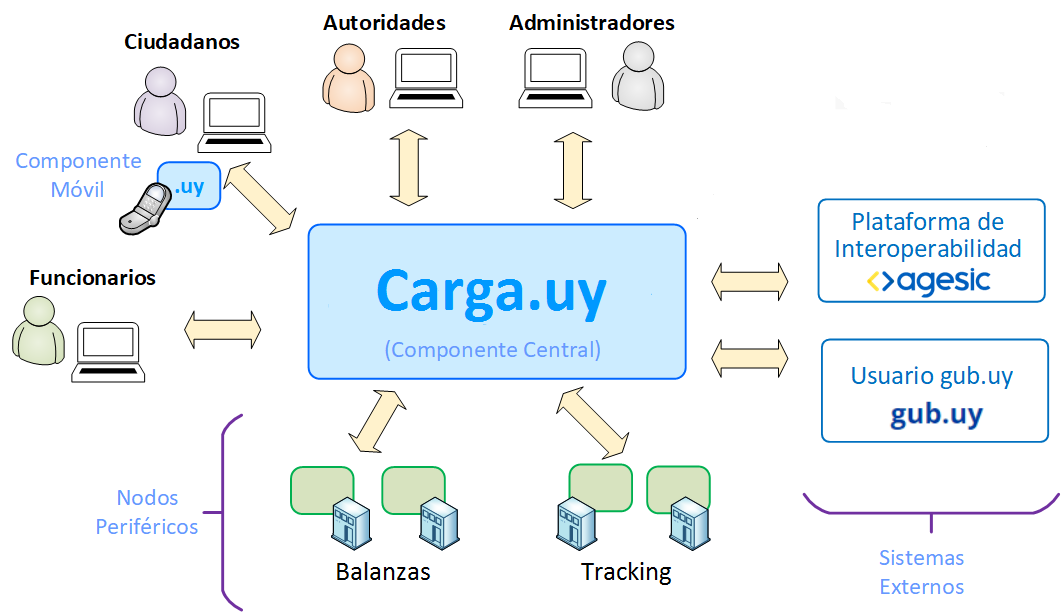
\includegraphics[width=15cm]{figures/descripcion-general.png}
    \caption{Descripción general de carga.uy}
    \label{fig:descr_general_plat}
\end{figure}

\subsection{Modelo Conceptual}

Los conceptos centrales son Usuario (Ciudadano, Funcionario, Administrador y Autoridad), Rol, Responsable, Chofer, Empresa, Vehículo, Permiso, ITV, Guía, Rubro, Tipo de Carga, Viaje, Evento (de viaje, incidente y de posición), Balanza, Peaje, Pesaje, Norma de Fiscalización, Caso de Fiscalización, Evidencia, Notificación, Descargo, Resolución, Pista de Auditoría e Informe. Un responsable representa a una empresa, que posee vehículos habilitados por un permiso e inspeccionados mediante la ITV. La empresa emite Guías que amparan viajes, asignados a un vehículo y conducidos por un chofer. Los eventos y pesajes asociados a los viajes constituyen evidencia para que las normas de fiscalización detecten posibles incumplimientos. Cada detección genera un caso que se notifica a la empresa, puede recibir un descargo y es resuelto por un funcionario, quedando sus acciones registradas en la pista de auditoría.

Los usuarios que se autentican con el mecanismo interno (autoridades y administradores) se agrupan bajo Usuario Backoffice, que es el único que guarda credenciales propias; funcionarios y ciudadanos se autentican con Usuario gub.uy.

\pendiente{en el monitoreo el tutor sugirió evaluar que la balanza tenga la ubicación y que Peaje y Balanza queden en relación 1 a 1, y dejar el modelo de dominio en pausa. Decidir si se aplica antes de la entrega.}

\begin{sidewaysfigure}
    \centering
    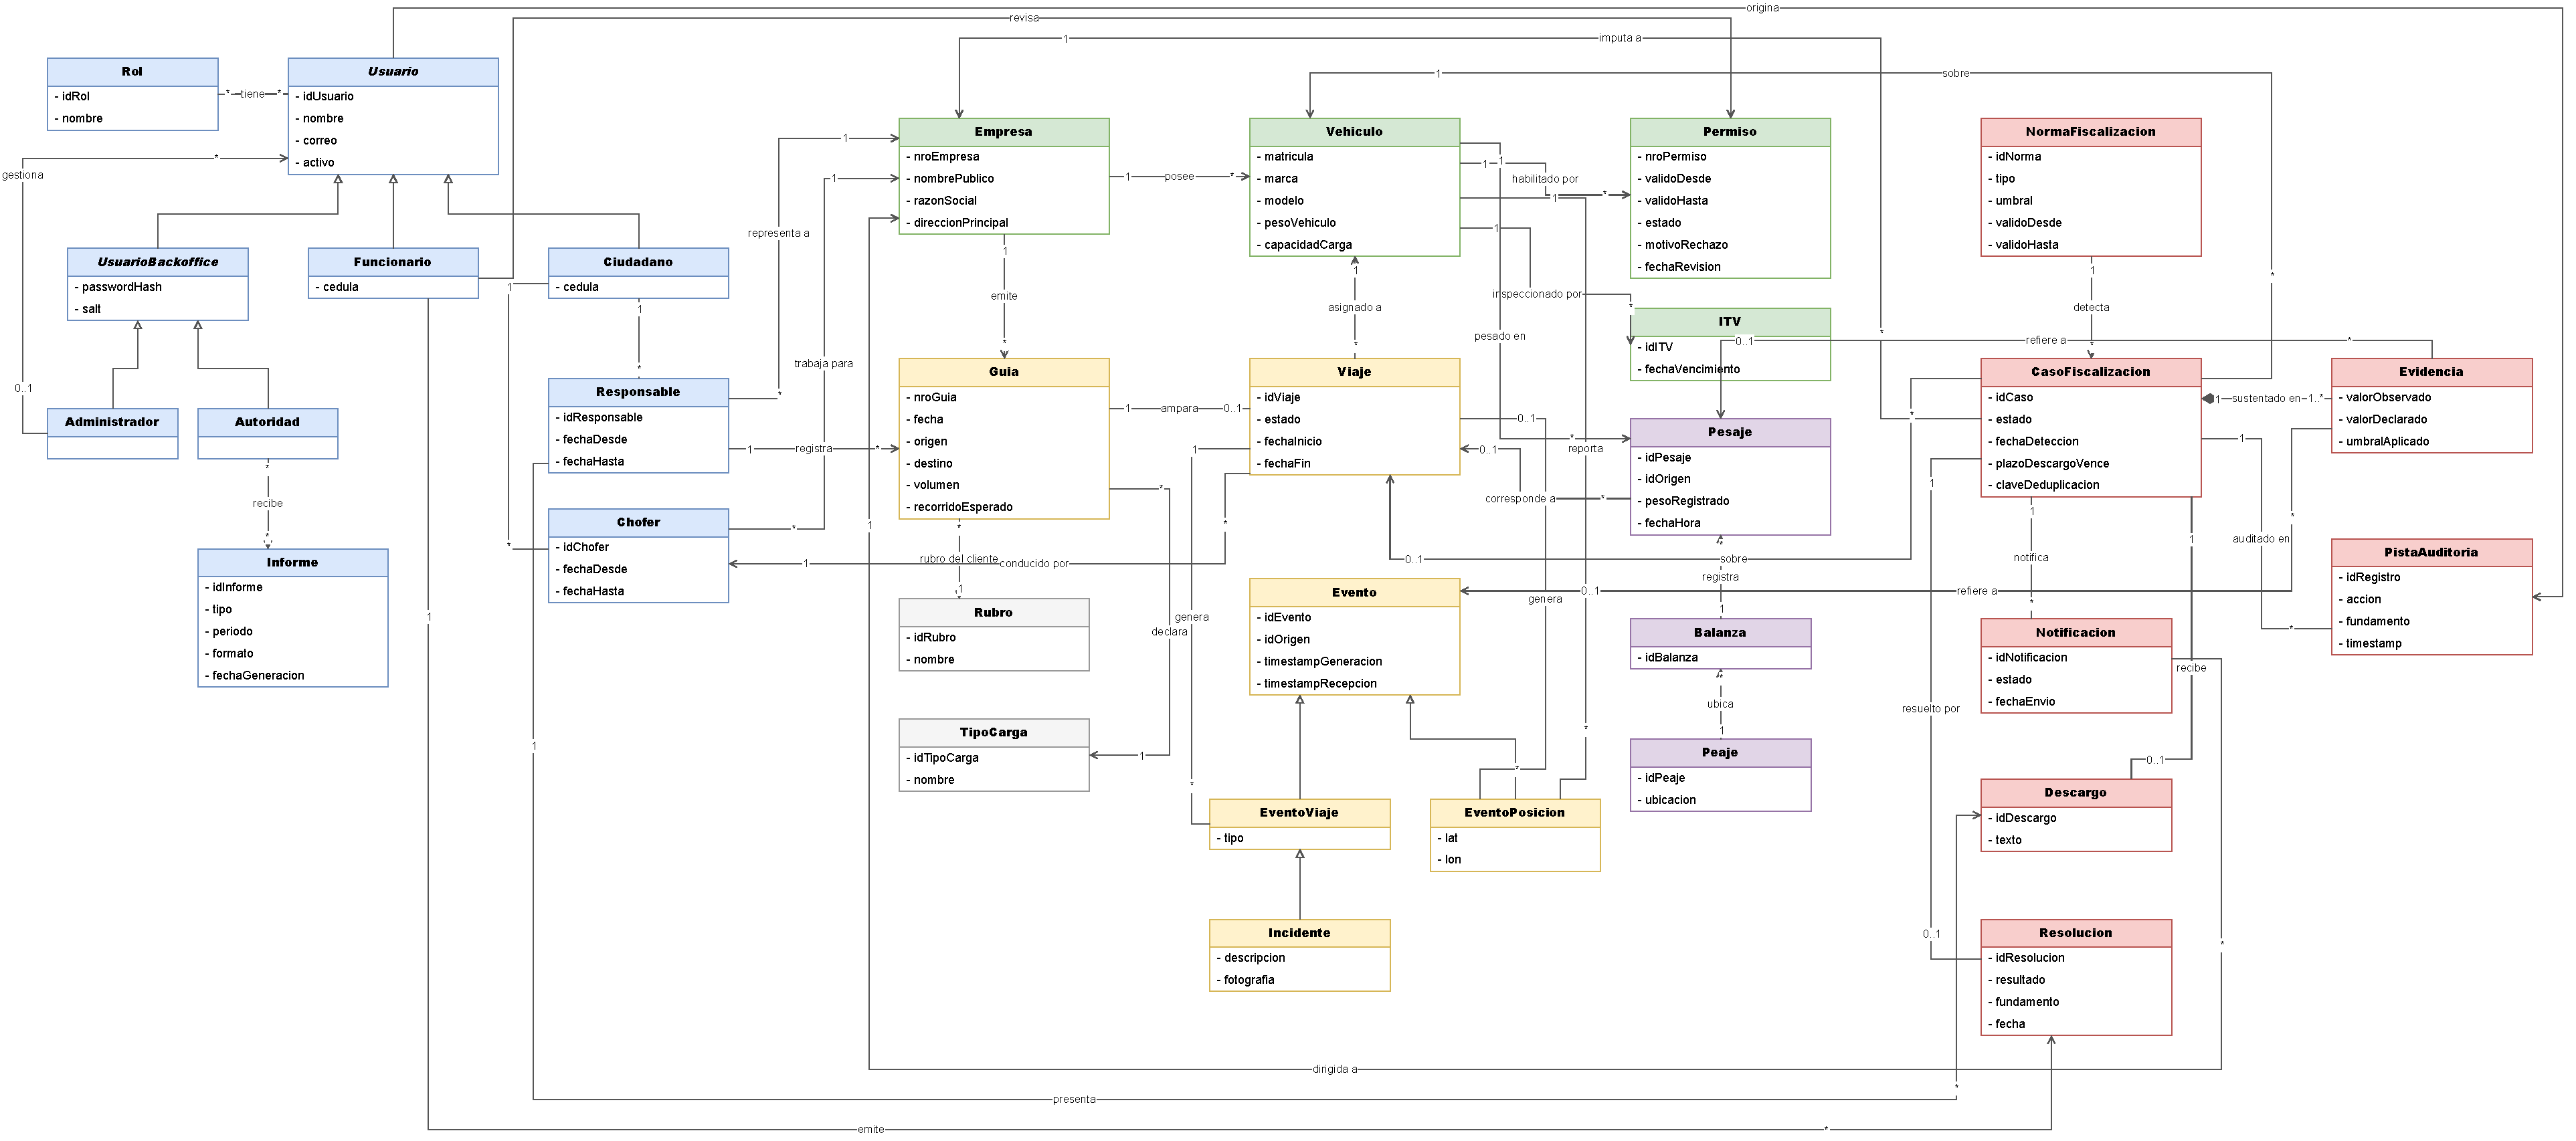
\includegraphics[width=0.98\textheight]{figures/modelo-conceptual.pdf}
    \caption{Modelo conceptual de carga.uy}
    \label{fig:modelo_conceptual}
\end{sidewaysfigure}

\section{Vista de Casos de Uso}\label{sec:vista-casos-de-uso}

La Vista de Casos de Uso se centra en los aspectos funcionales de la plataforma. En esta vista se presentan los actores así como los casos de uso de la plataforma, y se detallan los casos de uso que se consideran críticos para la arquitectura \cite{LINS2026}.

\subsection{Actores}

\begin{itemize}
    \item \textbf{Público general y empresa cliente:} consulta información pública y valida permisos de empresas transportistas.
    \item \textbf{Ciudadano responsable de empresa:} administra el perfil de la empresa, vehículos, guías, viajes e infracciones.
    \item \textbf{Chofer:} consulta el viaje asignado y registra sus eventos desde la aplicación móvil.
    \item \textbf{Funcionario del MTOP:} gestiona empresas y fiscaliza permisos, vehículos, viajes, pesajes e infracciones.
    \item \textbf{Autoridad del MTOP:} consulta el tablero de indicadores y exporta reportes.
    \item \textbf{Administrador:} gestiona usuarios, roles, nodos periféricos y parámetros de fiscalización.
    \item \textbf{Usuario gub.uy:} autentica ciudadanos y funcionarios.
    \item \textbf{Plataforma de Interoperabilidad:} proporciona datos de ciudadanos mediante servicios de organismos públicos.
    \item \textbf{Sistema de Balanzas:} devuelve los pesajes de un vehículo para una fecha determinada.
    \item \textbf{Sistema de Tracking:} envía de forma continua las posiciones de los vehículos durante los viajes.
\end{itemize}

\subsection{Diagrama de Casos de Uso}

En esta sección se utilizan Diagramas de Casos de Uso UML para presentar los casos de uso de la plataforma, indicando cuáles se consideran críticos para la arquitectura. Los casos críticos son CU-01, CU-07, CU-09, CU-10, CU-11, CU-16 y CU-19; el CU-19 se incorporó a pedido del tutor por su complejidad.

\begin{figure}[H]
    \centering
    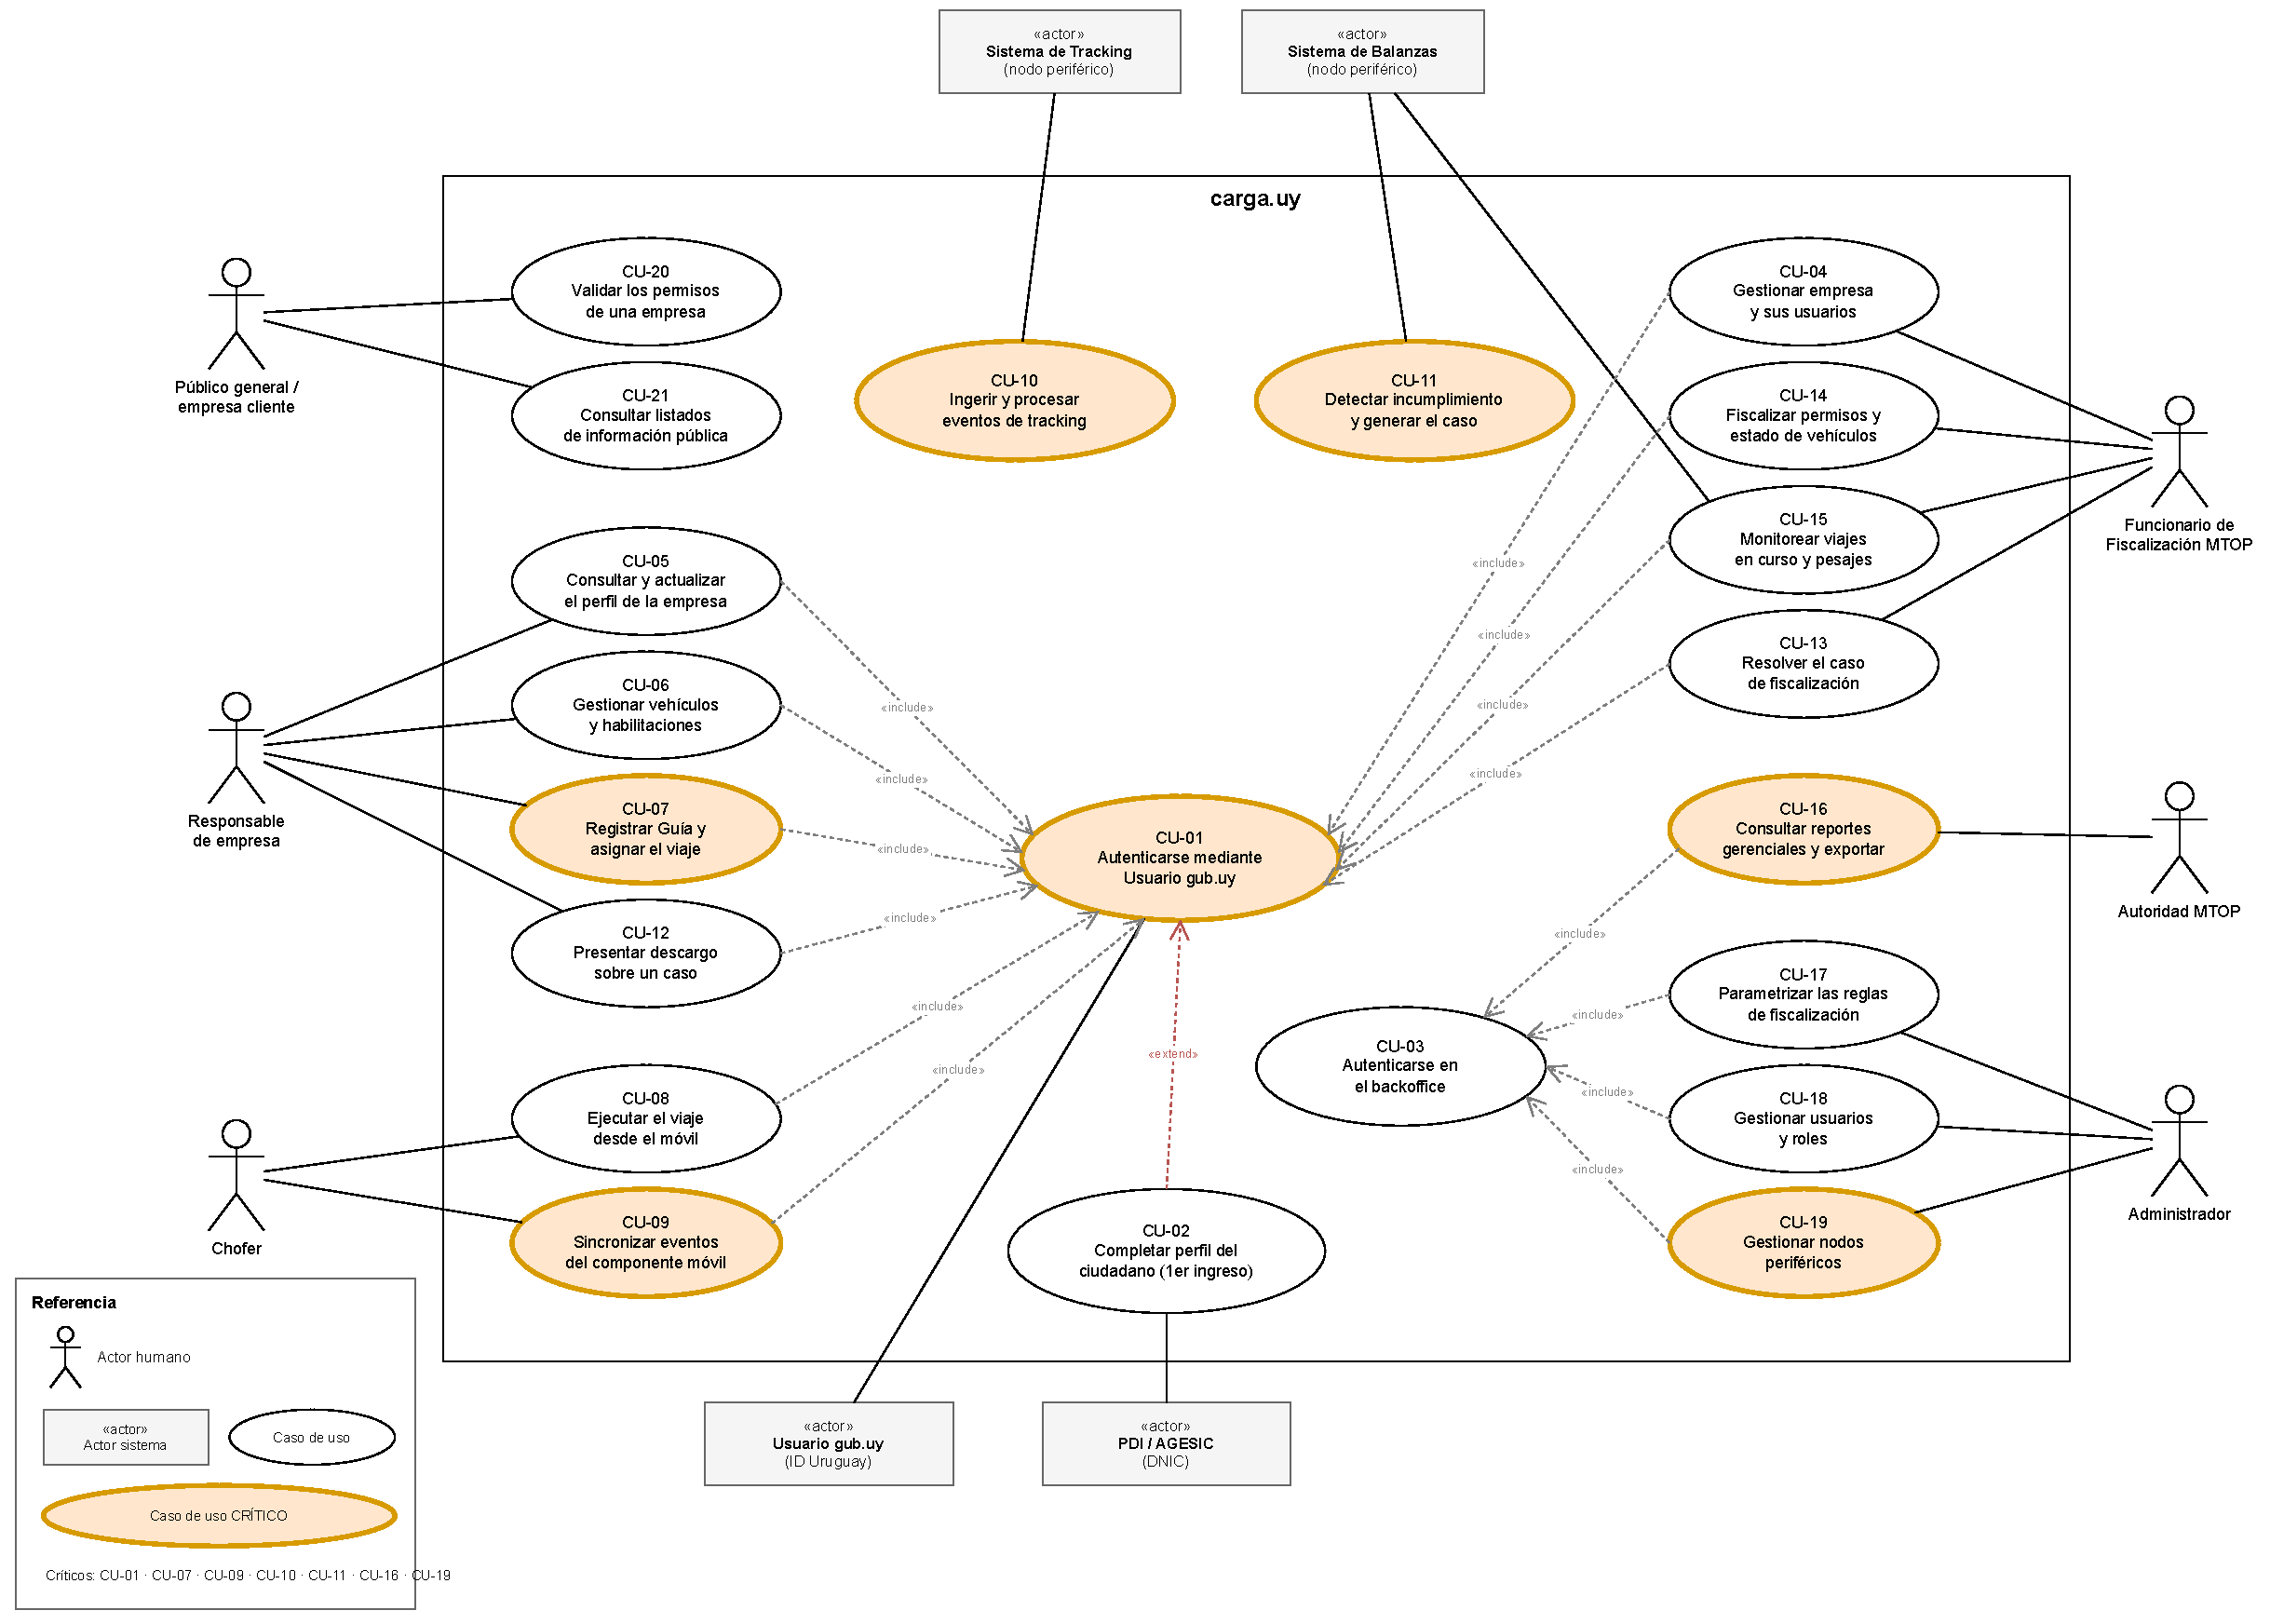
\includegraphics[width=\textwidth]{figures/casos-de-uso.pdf}
    \caption{Vista de Casos de Uso}
    \label{fig:usecases}
\end{figure}

La Tabla \ref{tab:cu-criticos} muestra qué componentes de la vista lógica (Sección \ref{sec:vista-logica}) intervienen en cada caso de uso crítico.

\begin{table}[H]
    \small
    \centering
    \caption{Componentes que intervienen en cada caso de uso crítico}
    \label{tab:cu-criticos}
    \begin{tabular}{|p{4.2cm}|p{11.6cm}|}
        \hline
        \textbf{Caso de uso} & \textbf{Componentes} \\
        \hline
        CU-01 Autenticarse mediante Usuario gub.uy & Frontoffice, API REST, Servicios de Negocio, Adaptador gub.uy, Persistencia y Usuario gub.uy. \\
        \hline
        CU-07 Registrar Guía y asignar el viaje & Frontoffice, Servicios de Negocio y Persistencia. \\
        \hline
        CU-09 Sincronizar los eventos del componente móvil & Componente Móvil y su persistencia local, API REST, Servicios de Negocio y Persistencia. \\
        \hline
        CU-10 Ingerir y procesar eventos de tracking & Nodo Periférico Tracking, Mensajería, Ingesta de Eventos, Persistencia y Motor de Fiscalización. \\
        \hline
        CU-11 Detectar un incumplimiento y generar el caso & Ingesta de Eventos, Motor de Fiscalización, Adaptador Balanzas, Nodo Periférico Balanzas, Persistencia, Notificaciones y Servicio de correo. \\
        \hline
        CU-16 Consultar reportes gerenciales y exportarlos & Backoffice, Generación de Reportes y Persistencia. \\
        \hline
        CU-19 Gestionar nodos periféricos & Backoffice, Servicios de Negocio y Persistencia; el registro de nodos condiciona además al Adaptador Balanzas y a la Ingesta de Eventos. \\
        \hline
    \end{tabular}
\end{table}

\pendiente{explicar el criterio con el que se eligieron los casos críticos. La plantilla propone dos: que intervenga el mayor número posible de componentes de la arquitectura y que intervengan los componentes críticos o más complejos.}

\FloatBarrier

\subsection{Funcionalidades Obligatorias}

\subsubsection{Frontoffice público}

\begin{enumerate}
    \item Autenticación mediante Usuario gub.uy.
    \item Validación de permisos de empresas transportistas.
    \item Consulta de listados de información pública agregada.
\end{enumerate}

\subsubsection{Frontoffice de empresas transportistas}

\begin{enumerate}
    \item \textbf{Perfil del ciudadano:} almacenar el correo electrónico y el número de cédula la primera vez que el usuario se autentica.
    \item \textbf{Perfil de la empresa:} consultar y actualizar nombre público, razón social, número de empresa y dirección principal.
    \item \textbf{Gestión de vehículos:} registrar matrícula, marca, modelo, peso, capacidad de carga, Permiso Nacional de Circulación e Inspección Técnica Vehicular.
    \item \textbf{Gestión de viajes:} ingresar guías con rubro del cliente, volumen, fecha, origen y destino, y asignarlas a un vehículo y un chofer.
    \item \textbf{Gestión de infracciones:} consultar infracciones y su evidencia, y presentar descargos dentro del plazo establecido.
\end{enumerate}

\subsubsection{Componente móvil}

\begin{enumerate}
    \item Autenticación mediante Usuario gub.uy.
    \item Consulta de la Guía y del viaje asignado al chofer.
    \item Registro del comienzo y finalización del viaje, cargas o descargas parciales e incidentes con fotografía opcional.
    \item Operación sin conectividad: la Guía debe estar disponible localmente; los eventos deben persistirse y sincronizarse al recuperar la conexión; cada evento debe tener un identificador generado en el dispositivo para evitar duplicados; y se debe definir una política de resolución de conflictos.
\end{enumerate}

\subsubsection{Frontoffice de funcionarios}

\begin{enumerate}
    \item Autenticación mediante Usuario gub.uy.
    \item Gestión de empresas de transporte.
    \item Fiscalización de permisos e ITV de los vehículos.
    \item Monitoreo de viajes en curso y finalizados, posiciones y pesajes.
    \item Gestión de casos de fiscalización: consultar evidencia y descargos, y confirmar o desestimar la infracción registrando el fundamento.
\end{enumerate}

\subsubsection{Backoffice de autoridades y administradores}

\begin{enumerate}
    \item Autenticación mediante un mecanismo interno y autorización basada en roles.
    \item Tablero para autoridades con cantidad de empresas y vehículos habilitados, viajes por período, volumen transportado por rubro, infracciones por tipo y tasa de confirmación.
    \item Filtrado de reportes por tipo de carga, ubicación y período, con exportación en al menos dos formatos.
    \item Gestión de usuarios, roles y nodos periféricos.
    \item Parametrización, sin redespliegue, de los umbrales de exceso de carga y desvío de ruta.
\end{enumerate}

\subsection{Fiscalización Automática}

La plataforma debe detectar como mínimo:

\begin{itemize}
    \item \textbf{Exceso de carga:} el pesaje supera el peso del vehículo más su capacidad declarada.
    \item \textbf{Vehículo sin habilitación vigente:} el permiso o la ITV están vencidos a la fecha del viaje.
    \item \textbf{Viaje sin Guía:} se recibe tracking o un pesaje para un vehículo sin un viaje asignado y en curso.
    \item \textbf{Desvío de ruta:} el recorrido reportado se aparta significativamente del trayecto esperado entre el origen y el destino declarados.
\end{itemize}

Cada detección genera un caso cuyo ciclo de vida es \emph{detectada}, \emph{notificada}, \emph{en descargo} y, finalmente, \emph{confirmada} o \emph{desestimada}. La detección debe ser automática y asincrónica; las transiciones deben estar controladas; la empresa debe ser notificada; las acciones de los funcionarios deben quedar auditadas; y el reprocesamiento de un evento no debe crear casos duplicados.

\FloatBarrier

\subsection{Casos de Uso Críticos}

Cada caso de uso crítico se describe en una de las siguientes subsecciones, con su descripción, sus precondiciones, el flujo principal, los flujos alternativos relevantes y sus postcondiciones.

\subsubsection{CU-01 Autenticarse mediante Usuario gub.uy}\label{sec:cu-01}
\begin{table}[H]
\small
\setlength{\tabcolsep}{8pt}
\renewcommand{\arraystretch}{1.1}
\centering
\begin{tabular}{|p{15.8cm}|}
\hline
\textbf{\underline{Actor principal:}} Ciudadano (responsable o chofer) o Funcionario MTOP. \\ \hline
\textbf{\underline{Actor secundario:}} Usuario gub.uy (ID Uruguay). \\ \hline
\textbf{\underline{Canales:}} Frontoffice web y componente móvil. \\ \hline
\textbf{\underline{Descripción:}} Permite que el usuario se identifique mediante Usuario gub.uy. Una vez autenticado, carga.uy crea la sesión y determina los permisos que le corresponden. \\ \hline
\textbf{\underline{Precondición:}} El usuario posee un Usuario gub.uy vigente. \\ \hline
\textbf{\underline{Flujo principal:}}\par
\begin{enumerate}[leftmargin=*,topsep=2pt,itemsep=1pt,parsep=0pt,partopsep=0pt]
    \item El usuario solicita ingresar.
    \item El sistema lo redirige a Usuario gub.uy.
    \item El usuario completa la autenticación.
    \item Usuario gub.uy devuelve el resultado.
    \item El sistema valida la respuesta y obtiene cédula y correo.
    \item Busca un perfil local asociado a la cédula.
    \item Establece la sesión, resuelve roles y permisos, y redirige al usuario.
    \item Registra el ingreso con identificador de correlación.
\end{enumerate} \\ \hline
\textbf{\underline{Alternativas y excepciones:}}\par
\begin{itemize}[leftmargin=*,topsep=2pt,itemsep=1pt,parsep=0pt,partopsep=0pt]
    \item Si no existe perfil local, se crea antes de establecer la sesión.
    \item Un ciudadano sin empresa asociada accede solamente a funciones públicas.
    \item Una autenticación cancelada, fallida, inválida o vencida no crea sesión.
    \item Si gub.uy no responde, las funcionalidades públicas siguen disponibles.
    \item En el móvil, una sesión previa válida permite operar sin conexión.
\end{itemize} \\ \hline
\textbf{\underline{Postcondiciones:}} Existe una sesión con identidad, roles y permisos resueltos, o no existe sesión. El evento queda registrado y no se almacenan credenciales del usuario. \\ \hline
\end{tabular}
\end{table}

\subsubsection{CU-07 Registrar Guía y asignar el viaje}\label{sec:cu-07}
\begin{table}[H]
\small
\setlength{\tabcolsep}{8pt}
\renewcommand{\arraystretch}{1.1}
\centering
\begin{tabular}{|p{15.8cm}|}
\hline
\textbf{\underline{Actor principal:}} Responsable de empresa. \\ \hline
\textbf{\underline{Descripción:}} Permite registrar la Guía de un viaje de carga y asignarla a un vehículo y a un chofer de la empresa. \\ \hline
\textbf{\underline{Precondiciones:}} El responsable está autenticado, la empresa está activa y existen al menos un vehículo y un chofer disponibles. \\ \hline
\textbf{\underline{Flujo principal:}}\par
\begin{enumerate}[leftmargin=*,topsep=2pt,itemsep=1pt,parsep=0pt,partopsep=0pt]
    \item El responsable selecciona “nueva Guía”.
    \item Ingresa rubro, volumen y tipo de carga, fecha, origen y destino.
    \item El sistema valida los datos y calcula el recorrido esperado.
    \item Genera una Guía única en estado \emph{registrada}.
    \item El responsable selecciona un vehículo habilitado y un chofer.
    \item El sistema valida que no existan viajes solapados.
    \item Crea el viaje en estado \emph{asignado} y lo publica en el móvil.
    \item Notifica al chofer.
\end{enumerate} \\ \hline
\textbf{\underline{Alternativas y excepciones:}}\par
\begin{itemize}[leftmargin=*,topsep=2pt,itemsep=1pt,parsep=0pt,partopsep=0pt]
    \item Se rechaza la asignación si el Permiso o la ITV no están vigentes.
    \item Se rechaza si la capacidad del vehículo es insuficiente o existe un solapamiento.
    \item Un origen o destino no georreferenciable debe corregirse.
    \item Una cancelación previa al inicio deja el viaje en estado \emph{cancelado}.
\end{itemize} \\ \hline
\textbf{\underline{Postcondiciones:}} Existe una Guía con viaje, vehículo, chofer y recorrido esperado. El viaje queda disponible para el chofer y sirve como referencia para tracking y pesajes. \\ \hline
\end{tabular}
\end{table}

\subsubsection{CU-09 Sincronizar los eventos del componente móvil}\label{sec:cu-09}
\begin{table}[H]
\small
\setlength{\tabcolsep}{8pt}
\renewcommand{\arraystretch}{1.1}
\centering
\begin{tabular}{|p{15.8cm}|}
\hline
\textbf{\underline{Actor principal:}} Chofer. \\ \hline
\textbf{\underline{Descripción:}} Sincroniza los eventos registrados sin conexión, evita duplicados y trata los conflictos producidos si el viaje cambió mientras el dispositivo estaba fuera de línea. \\ \hline
\textbf{\underline{Precondiciones:}} Existen eventos pendientes, se recuperó la conectividad y la sesión está vigente o pudo renovarse. \\ \hline
\textbf{\underline{Flujo principal:}}\par
\begin{enumerate}[leftmargin=*,topsep=2pt,itemsep=1pt,parsep=0pt,partopsep=0pt]
    \item La aplicación ordena y envía los eventos pendientes con sus identificadores.
    \item El componente central verifica si cada identificador ya fue procesado.
    \item Aplica los eventos nuevos respetando la máquina de estados.
    \item Descarta los eventos conocidos sin repetir sus efectos.
    \item Responde con el resultado y la versión actual del viaje.
    \item La aplicación elimina de la cola los eventos confirmados.
\end{enumerate} \\ \hline
\textbf{\underline{Alternativas y excepciones:}}\par
\begin{itemize}[leftmargin=*,topsep=2pt,itemsep=1pt,parsep=0pt,partopsep=0pt]
    \item Los eventos de un viaje cancelado o reasignado se conservan como evidencia y se marca el conflicto.
    \item Los eventos no confirmados se reenvían si la sincronización se interrumpe.
    \item Ante recuperaciones simultáneas de conectividad, los eventos permanecen pendientes hasta poder procesarse.
\end{itemize} \\ \hline
\textbf{\underline{Postcondiciones:}} Cada evento produce un único efecto; no existen duplicados y los conflictos quedan marcados sin pérdida de información. \\ \hline
\end{tabular}
\end{table}

\subsubsection{CU-10 Ingerir y procesar eventos de tracking}\label{sec:cu-10}
\begin{table}[H]
\small
\setlength{\tabcolsep}{8pt}
\renewcommand{\arraystretch}{1.1}
\centering
\begin{tabular}{|p{15.8cm}|}
\hline
\textbf{\underline{Actor principal:}} Sistema de Tracking (nodo periférico). \\ \hline
\textbf{\underline{Descripción:}} Recibe las posiciones enviadas por los vehículos durante un viaje y las utiliza para reconstruir la ruta recorrida. \\ \hline
\textbf{\underline{Precondiciones:}} El nodo de tracking está registrado y habilitado, y el mecanismo de mensajería está disponible. \\ \hline
\textbf{\underline{Flujo principal:}}\par
\begin{enumerate}[leftmargin=*,topsep=2pt,itemsep=1pt,parsep=0pt,partopsep=0pt]
    \item El nodo publica eventos con vehículo, coordenadas, marca de tiempo e identificador.
    \item El componente central recibe y encola los eventos.
    \item Un consumidor toma los eventos de la cola.
    \item Descarta los identificadores ya procesados.
    \item Asocia cada evento al viaje que estaba en curso cuando se generó.
    \item Ordena las posiciones por su momento de generación.
    \item Actualiza las métricas de procesamiento.
\end{enumerate} \\ \hline
\textbf{\underline{Alternativas y excepciones:}}\par
\begin{itemize}[leftmargin=*,topsep=2pt,itemsep=1pt,parsep=0pt,partopsep=0pt]
    \item Un vehículo sin viaje en curso al generarse el evento dispara la regla \emph{viaje sin Guía}.
    \item Ante saturación, los eventos permanecen encolados y pueden agregarse consumidores.
    \item Si el nodo no responde, el componente central continúa funcionando.
    \item Los eventos tardíos se incorporan a la ruta histórica y vuelven a evaluar las reglas.
\end{itemize} \\ \hline
\textbf{\underline{Postcondiciones:}} La ruta contiene las posiciones recibidas, ordenadas y sin duplicados, sin pérdida dentro del volumen objetivo. \\ \hline
\end{tabular}
\end{table}

\textbf{Asociación de posiciones a viajes.} Cada posición se asocia al viaje que el vehículo tenía en curso a la hora en que se generó la posición, y no al que tiene cuando la posición llega al componente central. Las horas de inicio y fin de cada viaje son las que registró el chofer en la aplicación móvil.

Por ejemplo, si un viaje va de 10:00 a 12:00 y el vehículo pierde cobertura desde las 11:30, las posiciones de 11:30 a 12:00 pueden llegar a las 12:15, con el viaje ya finalizado. Con este criterio igual quedan en ese viaje. Si se mirara el estado del viaje al llegar cada posición, parecerían de un vehículo sin viaje y se abriría un caso falso de \emph{viaje sin Guía}.

Puede pasar también lo inverso: si el chofer inicia el viaje sin conexión, las posiciones llegan antes que el aviso de inicio. Cuando el aviso llega, esas posiciones se asocian al viaje y se vuelve a evaluar la regla \emph{viaje sin Guía}.

\subsubsection{CU-11 Detectar automáticamente un incumplimiento y generar el caso}\label{sec:cu-11}
\begin{table}[H]
\small
\setlength{\tabcolsep}{8pt}
\renewcommand{\arraystretch}{1.1}
\centering
\begin{tabular}{|p{15.8cm}|}
\hline
\textbf{\underline{Disparador:}} El procesamiento de un evento de tracking (CU-10) o del fin de un viaje registrado desde el móvil (CU-09); no tiene actor humano. \\ \hline
\textbf{\underline{Actores secundarios:}} Sistema de Balanzas y empresa transportista. \\ \hline
\textbf{\underline{Descripción:}} Cruza la información declarada con los datos de tracking y balanzas para detectar incumplimientos y generar el caso correspondiente. \\ \hline
\textbf{\underline{Precondiciones:}} Existen datos declarados y recibidos, y los umbrales de tolerancia están parametrizados. \\ \hline
\textbf{\underline{Flujo principal:}}\par
\begin{enumerate}[leftmargin=*,topsep=2pt,itemsep=1pt,parsep=0pt,partopsep=0pt]
    \item La detección se ejecuta en segundo plano.
    \item Si el evento es el fin de un viaje, consulta a Balanzas los pesajes del vehículo y evalúa el exceso de carga.
    \item Verifica la vigencia del Permiso y la ITV.
    \item Detecta actividad de vehículos sin Guía.
    \item Compara la ruta con el recorrido y los umbrales configurados.
    \item Comprueba que el hecho no haya generado otro caso.
    \item Crea el caso en estado \emph{detectada} y almacena la evidencia.
    \item Lo publica y solicita la notificación a la empresa; al confirmarse el envío, el caso pasa a \emph{notificada} e inicia el plazo de descargo.
    \item Registra la creación en la pista de auditoría.
\end{enumerate} \\ \hline
\textbf{\underline{Alternativas y excepciones:}}\par
\begin{itemize}[leftmargin=*,topsep=2pt,itemsep=1pt,parsep=0pt,partopsep=0pt]
    \item Si Balanzas no responde, la evaluación queda pendiente sin detener la plataforma.
    \item La evidencia nueva se agrega a un caso existente por el mismo hecho.
    \item No se determina un desvío con posiciones insuficientes.
    \item Una falla del correo no bloquea el caso y provoca un reintento.
\end{itemize} \\ \hline
\textbf{\underline{Postcondiciones:}} Existe un caso con evidencia, en estado \emph{notificada} o en \emph{detectada} hasta que se confirme el envío, sin duplicados y con su creación auditada. \\ \hline
\end{tabular}
\end{table}

\textbf{Consulta a balanzas.} La integración con balanzas es de solicitud--respuesta (R3): los pesajes no llegan solos, el componente central los pide por vehículo y fecha. Por eso el exceso de carga se evalúa cuando el viaje finaliza: el motor pide los pesajes de cada fecha del viaje y compara cada pesada del horario del viaje con el peso del vehículo más su capacidad declarada. La justificación está en la decisión DA10 (Tabla \ref{tab:da10}).

\subsubsection{CU-16 Consultar reportes gerenciales y exportarlos}\label{sec:cu-16}
\begin{table}[H]
\small
\setlength{\tabcolsep}{8pt}
\renewcommand{\arraystretch}{1.1}
\centering
\begin{tabular}{|p{15.8cm}|}
\hline
\textbf{\underline{Actor principal:}} Autoridad MTOP. \\ \hline
\textbf{\underline{Descripción:}} Permite consultar indicadores generales de operación y fiscalización, aplicar filtros y exportar los resultados. \\ \hline
\textbf{\underline{Precondición:}} La autoridad está autenticada en el backoffice con el rol correspondiente. \\ \hline
\textbf{\underline{Flujo principal:}}\par
\begin{enumerate}[leftmargin=*,topsep=2pt,itemsep=1pt,parsep=0pt,partopsep=0pt]
    \item La autoridad accede al dashboard.
    \item El sistema presenta los indicadores obligatorios.
    \item La autoridad filtra por carga, ubicación y período.
    \item El sistema recalcula los indicadores.
    \item La autoridad solicita una exportación en CSV o PDF.
    \item El sistema genera el archivo y lo pone a disposición.
\end{enumerate} \\ \hline
\textbf{\underline{Alternativas y excepciones:}}\par
\begin{itemize}[leftmargin=*,topsep=2pt,itemsep=1pt,parsep=0pt,partopsep=0pt]
    \item Un rango muy amplio genera una advertencia o una limitación del período.
    \item Una exportación grande se genera en segundo plano.
    \item Si no existen datos, se informa explícitamente.
    \item El umbral de agregación pública no limita los reportes internos del MTOP.
\end{itemize} \\ \hline
\textbf{\underline{Postcondiciones:}} La autoridad visualizó los indicadores y, si corresponde, obtuvo el archivo. El acceso quedó registrado. \\ \hline
\end{tabular}
\end{table}

\subsubsection{CU-19 Gestionar nodos periféricos}\label{sec:cu-19}
\begin{table}[H]
\small
\setlength{\tabcolsep}{8pt}
\renewcommand{\arraystretch}{1.1}
\centering
\begin{tabular}{|p{15.8cm}|}
\hline
\textbf{\underline{Actor principal:}} Administrador. \\ \hline
\textbf{\underline{Actores secundarios:}} Nodo Periférico Balanzas y Nodo Periférico Tracking. \\ \hline
\textbf{\underline{Canales:}} Backoffice web. \\ \hline
\textbf{\underline{Descripción:}} Permite registrar, consultar, modificar, habilitar, deshabilitar y dar de baja los nodos periféricos de balanzas y de tracking de los que la plataforma obtiene pesajes y posiciones. \\ \hline
\textbf{\underline{Precondiciones:}} El administrador está autenticado en el backoffice con el rol correspondiente y el componente periférico está desplegado. \\ \hline
\textbf{\underline{Flujo principal:}}\par
\begin{enumerate}[leftmargin=*,topsep=2pt,itemsep=1pt,parsep=0pt,partopsep=0pt]
    \item El administrador accede a la gestión de nodos y el sistema lista los nodos registrados con su tipo, punto de acceso y estado.
    \item Selecciona registrar un nodo e indica su tipo (balanzas o tracking), un identificador y su punto de acceso.
    \item El sistema valida que el identificador no esté en uso.
    \item Registra el nodo en estado \emph{deshabilitado}.
    \item El administrador solicita verificar la conectividad con el nodo.
    \item Si la verificación es exitosa, el administrador habilita el nodo.
    \item A partir de ese momento el nodo intercambia datos con el componente central.
\end{enumerate} \\ \hline
\textbf{\underline{Alternativas y excepciones:}}\par
\begin{itemize}[leftmargin=*,topsep=2pt,itemsep=1pt,parsep=0pt,partopsep=0pt]
    \item Si el identificador ya está en uso, se rechaza el registro.
    \item Si la verificación falla, el nodo permanece deshabilitado y se informa el motivo.
    \item Modificar el punto de acceso de un nodo habilitado lo vuelve a \emph{deshabilitado} hasta una nueva verificación.
    \item Deshabilitar un nodo de balanzas deja pendiente la evaluación de exceso de carga sin detener la plataforma.
    \item Deshabilitar un nodo de tracking hace que se descarten sus eventos y los viajes en curso quedan sin actualización de ruta.
    \item La baja es lógica: los pesajes y las posiciones que el nodo reportó siguen siendo evidencia de los casos generados.
\end{itemize} \\ \hline
\textbf{\underline{Postcondiciones:}} El nodo queda registrado con su tipo, punto de acceso y estado. Solo los nodos habilitados intercambian datos con el componente central y ninguna credencial queda en el repositorio. \\ \hline
\end{tabular}
\end{table}

La verificación de conectividad consulta el punto de acceso del nodo: a un nodo de balanzas se le hace una consulta de pesajes de prueba, y a un nodo de tracking se le consulta su estado (\texttt{/health}), que indica si está conectado a la mensajería.

\section{Vista de Restricciones}\label{sec:vista-de-restricciones}

La Vista de Restricciones describe restricciones que deben respetarse tanto en el proceso de desarrollo como en el producto \cite{Perovich2003}. Las restricciones de \solucion surgen de la letra del laboratorio \cite{LINS2026} y se agrupan en comunicación e integración, seguridad y protección de datos, y despliegue y operación. Se conservan los identificadores R1 a R17, a los que hacen referencia otras secciones del documento.

\begin{longtable}{|p{1.2cm}|p{14.3cm}|}
    \caption{Restricciones}\label{tab:restricciones}\\
    \hline
    \textbf{Id} & \textbf{Descripción} \\
    \hline
    \endfirsthead
    \hline
    \textbf{Id} & \textbf{Descripción} \\
    \hline
    \endhead
    \multicolumn{2}{|l|}{\textit{Comunicación e integración}} \\
    \hline
    R1 & La comunicación entre el componente central y la Plataforma de Interoperabilidad debe realizarse mediante servicios web SOAP. \\
    \hline
    R2 & La comunicación entre el componente móvil y el componente central debe realizarse mediante servicios web REST. \\
    \hline
    R3 & La integración con los nodos de balanzas debe ser sincrónica, de tipo solicitud--respuesta. \\
    \hline
    R4 & La integración con tracking debe ser asincrónica y unidireccional, apoyada en un mecanismo de mensajería. Se deben justificar la tecnología, el particionamiento y la política de entrega. \\
    \hline
    R5 & Los servicios no públicos de la PDI deben sustituirse por servicios que respeten, en la medida de lo posible, sus interfaces. \\
    \hline
    R6 & El procesamiento de eventos debe ser idempotente y admitir eventos duplicados o fuera de orden. \\
    \hline
    \multicolumn{2}{|l|}{\textit{Seguridad y protección de datos}} \\
    \hline
    R7 & Las contraseñas deben almacenarse mediante funciones hash con \textit{salt}. \\
    \hline
    R8 & Las interacciones con componentes periféricos, plataformas y el componente móvil deben utilizar HTTPS. \\
    \hline
    R9 & La autorización debe aplicarse en la capa de servicios y no solamente en la interfaz de usuario. \\
    \hline
    R10 & Las acciones de fiscalización deben registrarse en una pista de auditoría de solo agregado que no pueda modificarse ni eliminarse desde la aplicación. \\
    \hline
    R11 & Las credenciales, claves y certificados no deben almacenarse en el repositorio de código fuente. \\
    \hline
    R12 & La información pública debe presentarse agregada, sin permitir identificar a una empresa, vehículo o chofer particular, y se debe justificar el umbral de agregación. \\
    \hline
    \multicolumn{2}{|l|}{\textit{Despliegue y operación}} \\
    \hline
    R13 & Todos los componentes deben distribuirse contenerizados y el entorno completo debe iniciarse mediante un único comando documentado. \\
    \hline
    R14 & El componente central debe ejecutarse en la solución Elastic Cloud de ANTEL. \\
    \hline
    R15 & Los componentes periféricos deben ejecutarse en otras soluciones PaaS o IaaS. \\
    \hline
    R16 & El repositorio del proyecto en GitHub debe contar con integración continua que ejecute compilación, pruebas automatizadas y análisis estático ante cada modificación. \\
    \hline
    R17 & El pipeline de integración continua debe estar en estado exitoso al momento de la entrega final. \\
    \hline
\end{longtable}

\section{Vista de Atributos de Calidad}\label{sec:vista-calidad-de-servicio}

La Vista de Atributos de Calidad se centra en los requerimientos de atributos de calidad de la plataforma. Los atributos de calidad son propiedades medibles o comprobables de un sistema, que indican qué tan bien el sistema satisface las necesidades de las partes interesadas \cite{Bass2012}. Los requerimientos de esta sección surgen de la letra del laboratorio \cite{LINS2026} y se verifican mediante pruebas automatizadas, la prueba de performance y los mecanismos de observabilidad.

\begin{longtable}{|p{1.3cm}|p{2.7cm}|p{11.5cm}|}
    \caption{Atributos de Calidad}\label{tab:calidad}\\
    \hline
    \textbf{Id} & \textbf{Tipo} & \textbf{Descripción} \\
    \hline
    \endfirsthead
    \hline
    \textbf{Id} & \textbf{Tipo} & \textbf{Descripción} \\
    \hline
    \endhead
    \multicolumn{3}{|l|}{\textit{Seguridad}} \\
    \hline
    AC01 & Seguridad & Las contraseñas de los usuarios del backoffice las guarda el directorio LDAP con hash y \textit{salt} (R7); el componente central no las almacena. El directorio solo se accede por LDAPS. \\
    \hline
    AC02 & Seguridad & Las comunicaciones con los componentes periféricos, las plataformas externas y el componente móvil utilizan HTTPS (R8). \\
    \hline
    AC03 & Seguridad & La autorización se controla en la capa de servicios, con permisos asociados a roles (R9). \\
    \hline
    AC04 & Seguridad & La pista de auditoría permite reconstruir el usuario, la acción, el fundamento y la marca de tiempo de cada acción de fiscalización, y no puede modificarse ni eliminarse desde la aplicación (R10). Cada registro guarda el caso, la acción (crear, notificar, presentar descargo, confirmar o desestimar), el usuario y su rol, los estados anterior y nuevo, el fundamento y la fecha. Un disparador de PostgreSQL rechaza cualquier modificación o borrado de esos registros, aunque se intente desde fuera de la aplicación, y la pista referencia al caso solo por su identificador, para que borrar un caso no la borre en cascada. \\
    \hline
    AC05 & Seguridad & Las credenciales, claves y certificados se administran fuera del repositorio de código y de las imágenes de contenedor (R11). \\
    \hline
    AC06 & Privacidad & La información pública se publica agregada, respetando la normativa de protección de datos personales, con un umbral mínimo de agregación de \pendiente{definir y justificar el umbral (R12)}. \\
    \hline
    \multicolumn{3}{|l|}{\textit{Escalabilidad y performance}} \\
    \hline
    AC07 & Escalabilidad & El componente central escala horizontalmente en la capa web o de aplicaciones, sin estado de sesión almacenado localmente en las instancias. \\
    \hline
    AC08 & Performance & La plataforma sostiene, sin pérdida de eventos, un volumen de ingesta de tracking de \pendiente{estimar y justificar: cantidad de vehículos reportando en forma concurrente y frecuencia de reporte}, y picos de al menos tres veces ese volumen. \\
    \hline
    AC09 & Performance & El percentil 95 del tiempo de respuesta de las consultas del frontoffice es menor a 500 ms. \\
    \hline
    AC10 & Performance & Los tiempos de respuesta no se degradan a lo largo de la prueba de performance. \\
    \hline
    AC11 & Performance & La prueba de performance determina el punto de quiebre e identifica los cuellos de botella con evidencia de los mecanismos de observabilidad. \\
    \hline
    \multicolumn{3}{|l|}{\textit{Resiliencia e idempotencia}} \\
    \hline
    AC12 & Resiliencia & La indisponibilidad de un sistema externo o de un nodo periférico no provoca la indisponibilidad del componente central. \\
    \hline
    AC13 & Resiliencia & Las integraciones con sistemas externos y nodos periféricos aplican un tiempo de espera, reintentos y un corte ante fallas sostenidas, con un comportamiento degradado definido:
    \begin{itemize}[leftmargin=*,topsep=2pt,itemsep=1pt,parsep=0pt,partopsep=0pt]
        \item \textbf{Balanzas:} espera de 5 s, 2 reintentos a 1 s y 2 s, y corte por 60 s tras 5 fallas en 10 llamadas. La evaluación de exceso de carga queda pendiente y el resto de las reglas se evalúa igual.
        \item \textbf{PDI:} espera de 3 s, 1 reintento a 1 s, y corte por 30 s tras 5 fallas en 10 llamadas. El perfil del ciudadano se crea sin los datos de la PDI, que se completan en su próximo ingreso.
        \item \textbf{Usuario gub.uy:} espera de 5 s, sin reintentos. El ingreso falla con un mensaje y las sesiones ya iniciadas siguen funcionando.
        \item \textbf{Correo:} espera de 5 s y 3 reintentos a 1, 5 y 30 min. El caso avanza igual y la notificación se reintenta.
        \item \textbf{Servicio de rutas:} \pendiente{definir la espera, los reintentos y el corte}. La Guía se registra igual y el recorrido esperado queda pendiente hasta que se pueda obtener (CU-07).
        \item \textbf{Directorio LDAP:} \pendiente{definir la espera, los reintentos y el corte}. El ingreso al backoffice falla con un mensaje; las sesiones ya iniciadas siguen funcionando, porque el JWT no depende del directorio (DA03).
    \end{itemize}
    Los tiempos de espera, los reintentos y el corte de balanzas, PDI, Usuario gub.uy, el servicio de rutas y el directorio LDAP se implementan con la biblioteca de tolerancia a fallas que trae WildFly (MicroProfile Fault Tolerance), mediante anotaciones en los adaptadores (\texttt{@Timeout}, \texttt{@Retry}, \texttt{@CircuitBreaker}), y el comportamiento degradado con \texttt{@Fallback}. Los reintentos del correo, que se espacian en minutos, los realiza un temporizador que reprocesa los envíos pendientes. \\
    \hline
    AC14 & Resiliencia & Las pruebas incluyen un escenario con el Sistema de Balanzas indisponible y otro con la PDI sin responder. \\
    \hline
    AC15 & Idempotencia & Un evento recibido más de una vez no altera dos veces el estado del viaje ni genera casos de fiscalización adicionales. \\
    \hline
    AC16 & Consistencia & El orden de la ruta se reconstruye a partir del momento de generación de cada evento y no del orden de llegada. \\
    \hline
    AC17 & Resiliencia & Ante una saturación, las posiciones de tracking esperan en la cola y se procesan más tarde, sin perder ninguna. Para eso se usa el \emph{paging} del broker de mensajería (DA02, política \texttt{PAGE}): cuando la cola \texttt{queue\_tracking} llena su memoria, el broker guarda las posiciones nuevas en disco en lugar de descartarlas, y las procesa en orden a medida que se libera memoria. Se descartan tirar posiciones, porque la plataforma no debe perder eventos (AC08), y pedirle al nodo que reporte menos seguido, porque la frecuencia de reporte la fija el sistema de tracking, que es externo a la plataforma. \\
    \hline
    \multicolumn{3}{|l|}{\textit{Operación sin conectividad}} \\
    \hline
    AC18 & Disponibilidad & La aplicación móvil es utilizable sin conexión: conserva localmente la Guía descargada y los eventos pendientes. \\
    \hline
    AC19 & Idempotencia & Al recuperar la conectividad, la sincronización es idempotente: cada evento lleva un identificador generado en el dispositivo y su reenvío no produce duplicados. \\
    \hline
    AC20 & Consistencia & Ante un cambio hecho desde el frontoffice mientras el dispositivo estaba sin conexión, prevalece el componente central. El frontoffice solo modifica o elimina viajes que todavía no comenzaron, así que un evento sobre un viaje eliminado o reasignado queda en conflicto y no se aplica. Cada evento se procesa por separado y se registra con su resultado, sin pérdida de información, y la aplicación adopta el estado del viaje que devuelve el componente central (CU-09, Sección \ref{sec:cu-09}). Prevalece el componente central porque la asignación de los viajes la decide el responsable de la empresa. \\
    \hline
    \multicolumn{3}{|l|}{\textit{Observabilidad}} \\
    \hline
    AC21 & Observabilidad & Los componentes emiten logs estructurados que incluyen un identificador de correlación. El componente central y el nodo de tracking mandan sus logs con OpenTelemetry (OTLP) a la Plataforma de Observabilidad, como registros estructurados que llevan el identificador de la traza en curso: es el identificador de correlación, el mismo en el nodo y en el componente central para una misma posición. \\
    \hline
    AC22 & Observabilidad & El componente central expone métricas de eventos procesados, latencia de procesamiento, tamaño de las colas y errores por tipo, y endpoints de verificación de estado. Las métricas se exportan por OTLP con Micrometer: posiciones procesadas por resultado, errores por tipo, tiempo de procesamiento, espera en la cola y antigüedad de cada posición, mensajes y consumidores de la cola de tracking, y tiempo de respuesta de la API REST, con histogramas para calcular percentiles. Los endpoints de verificación de estado son \texttt{/health/live} y \texttt{/health/ready} del servidor de aplicaciones y \texttt{/api/salud}, que verifica PostgreSQL y el Almacén de Posiciones; la Plataforma de Observabilidad los consulta periódicamente. \\
    \hline
    AC23 & Observabilidad & Al menos un flujo que atraviesa el componente móvil, el componente central y un nodo periférico se traza de forma distribuida. Ese flujo es el fin de un viaje: el chofer lo registra en el móvil, el componente central lo recibe al sincronizar y el Motor de Fiscalización consulta los pesajes al nodo de Balanzas (CU-11, DA10). Además se traza la ingesta: el nodo de tracking abre una traza por cada lote que publica y su contexto viaja en cada mensaje, así que el procesamiento de cada posición en el componente central forma parte de esa traza. \\
    \hline
    AC24 & Observabilidad & El informe de la prueba de performance se apoya en la evidencia obtenida de logs, métricas y trazas. La plataforma incluye un tablero con esa evidencia para la ingesta, el nodo de tracking y la API REST. \\
    \hline
    \multicolumn{3}{|l|}{\textit{Pruebas y calidad del código}} \\
    \hline
    AC25 & Mantenibilidad & Las pruebas automatizadas cubren aproximadamente el 80~\% de la lógica, con al menos una prueba por servicio. La cobertura se mide con JaCoCo en el pipeline de integración continua. \\
    \hline
    AC26 & Corrección & Las pruebas cubren el ciclo de vida de los casos de fiscalización, verifican que no sean posibles transiciones de estado no previstas y comprueban la idempotencia del procesamiento de tracking y de la sincronización móvil. \\
    \hline
    AC27 & Mantenibilidad & El pipeline de integración continua ejecuta un análisis estático de calidad de código. \\
    \hline
\end{longtable}

\section{Vista Lógica}\label{sec:vista-logica}

La Vista Lógica describe la arquitectura lógica de la plataforma, utilizando varios niveles de refinamiento. En particular, se presentan y describen los principales componentes lógicos de la plataforma así como sus responsabilidades, dependencias e interacciones. Se utilizan Diagramas de Componentes UML \cite{Ambysoft2018b}, con el clasificador \enquote{subsystem} para la arquitectura general y \enquote{component} para los refinamientos.

\subsection{Arquitectura General del Sistema}

La plataforma se descompone en dos subsistemas principales: el Componente Móvil, utilizado por los choferes, y el Componente Central, que concentra el resto de las funcionalidades y se comunica con los nodos periféricos y los sistemas externos (Figura \ref{fig:vista_logica}).

El Componente Central se organiza en capas. La capa de presentación está formada por la API REST, consumida por el componente móvil, el Frontoffice, para el público, los ciudadanos y los funcionarios, y el Backoffice de autoridades y administradores. La capa de servicios y procesamiento agrupa los Servicios de Negocio (autorización, empresas, vehículos, viajes y casos), la Generación de Reportes, la Ingesta de Eventos y el Motor de Fiscalización, que es disparado por la ingesta para detectar incumplimientos de forma asincrónica. La Persistencia almacena los datos declarados, los eventos, los casos y la pista de auditoría. Finalmente, la capa de adaptadores e infraestructura aísla la integración con Usuario gub.uy (OpenID Connect), la PDI (SOAP), el servicio de correo (SMTP), el nodo de Balanzas (solicitud--respuesta) y el nodo de Tracking, cuyos eventos llegan de forma asincrónica mediante el subsistema de Mensajería.

El Componente Móvil cuenta con su propia persistencia local, donde mantiene la Guía descargada, el estado del viaje y la cola de eventos pendientes, lo que le permite operar sin conectividad y sincronizar con el Componente Central mediante REST sobre HTTPS.

\begin{figure}[H]
    \centering
    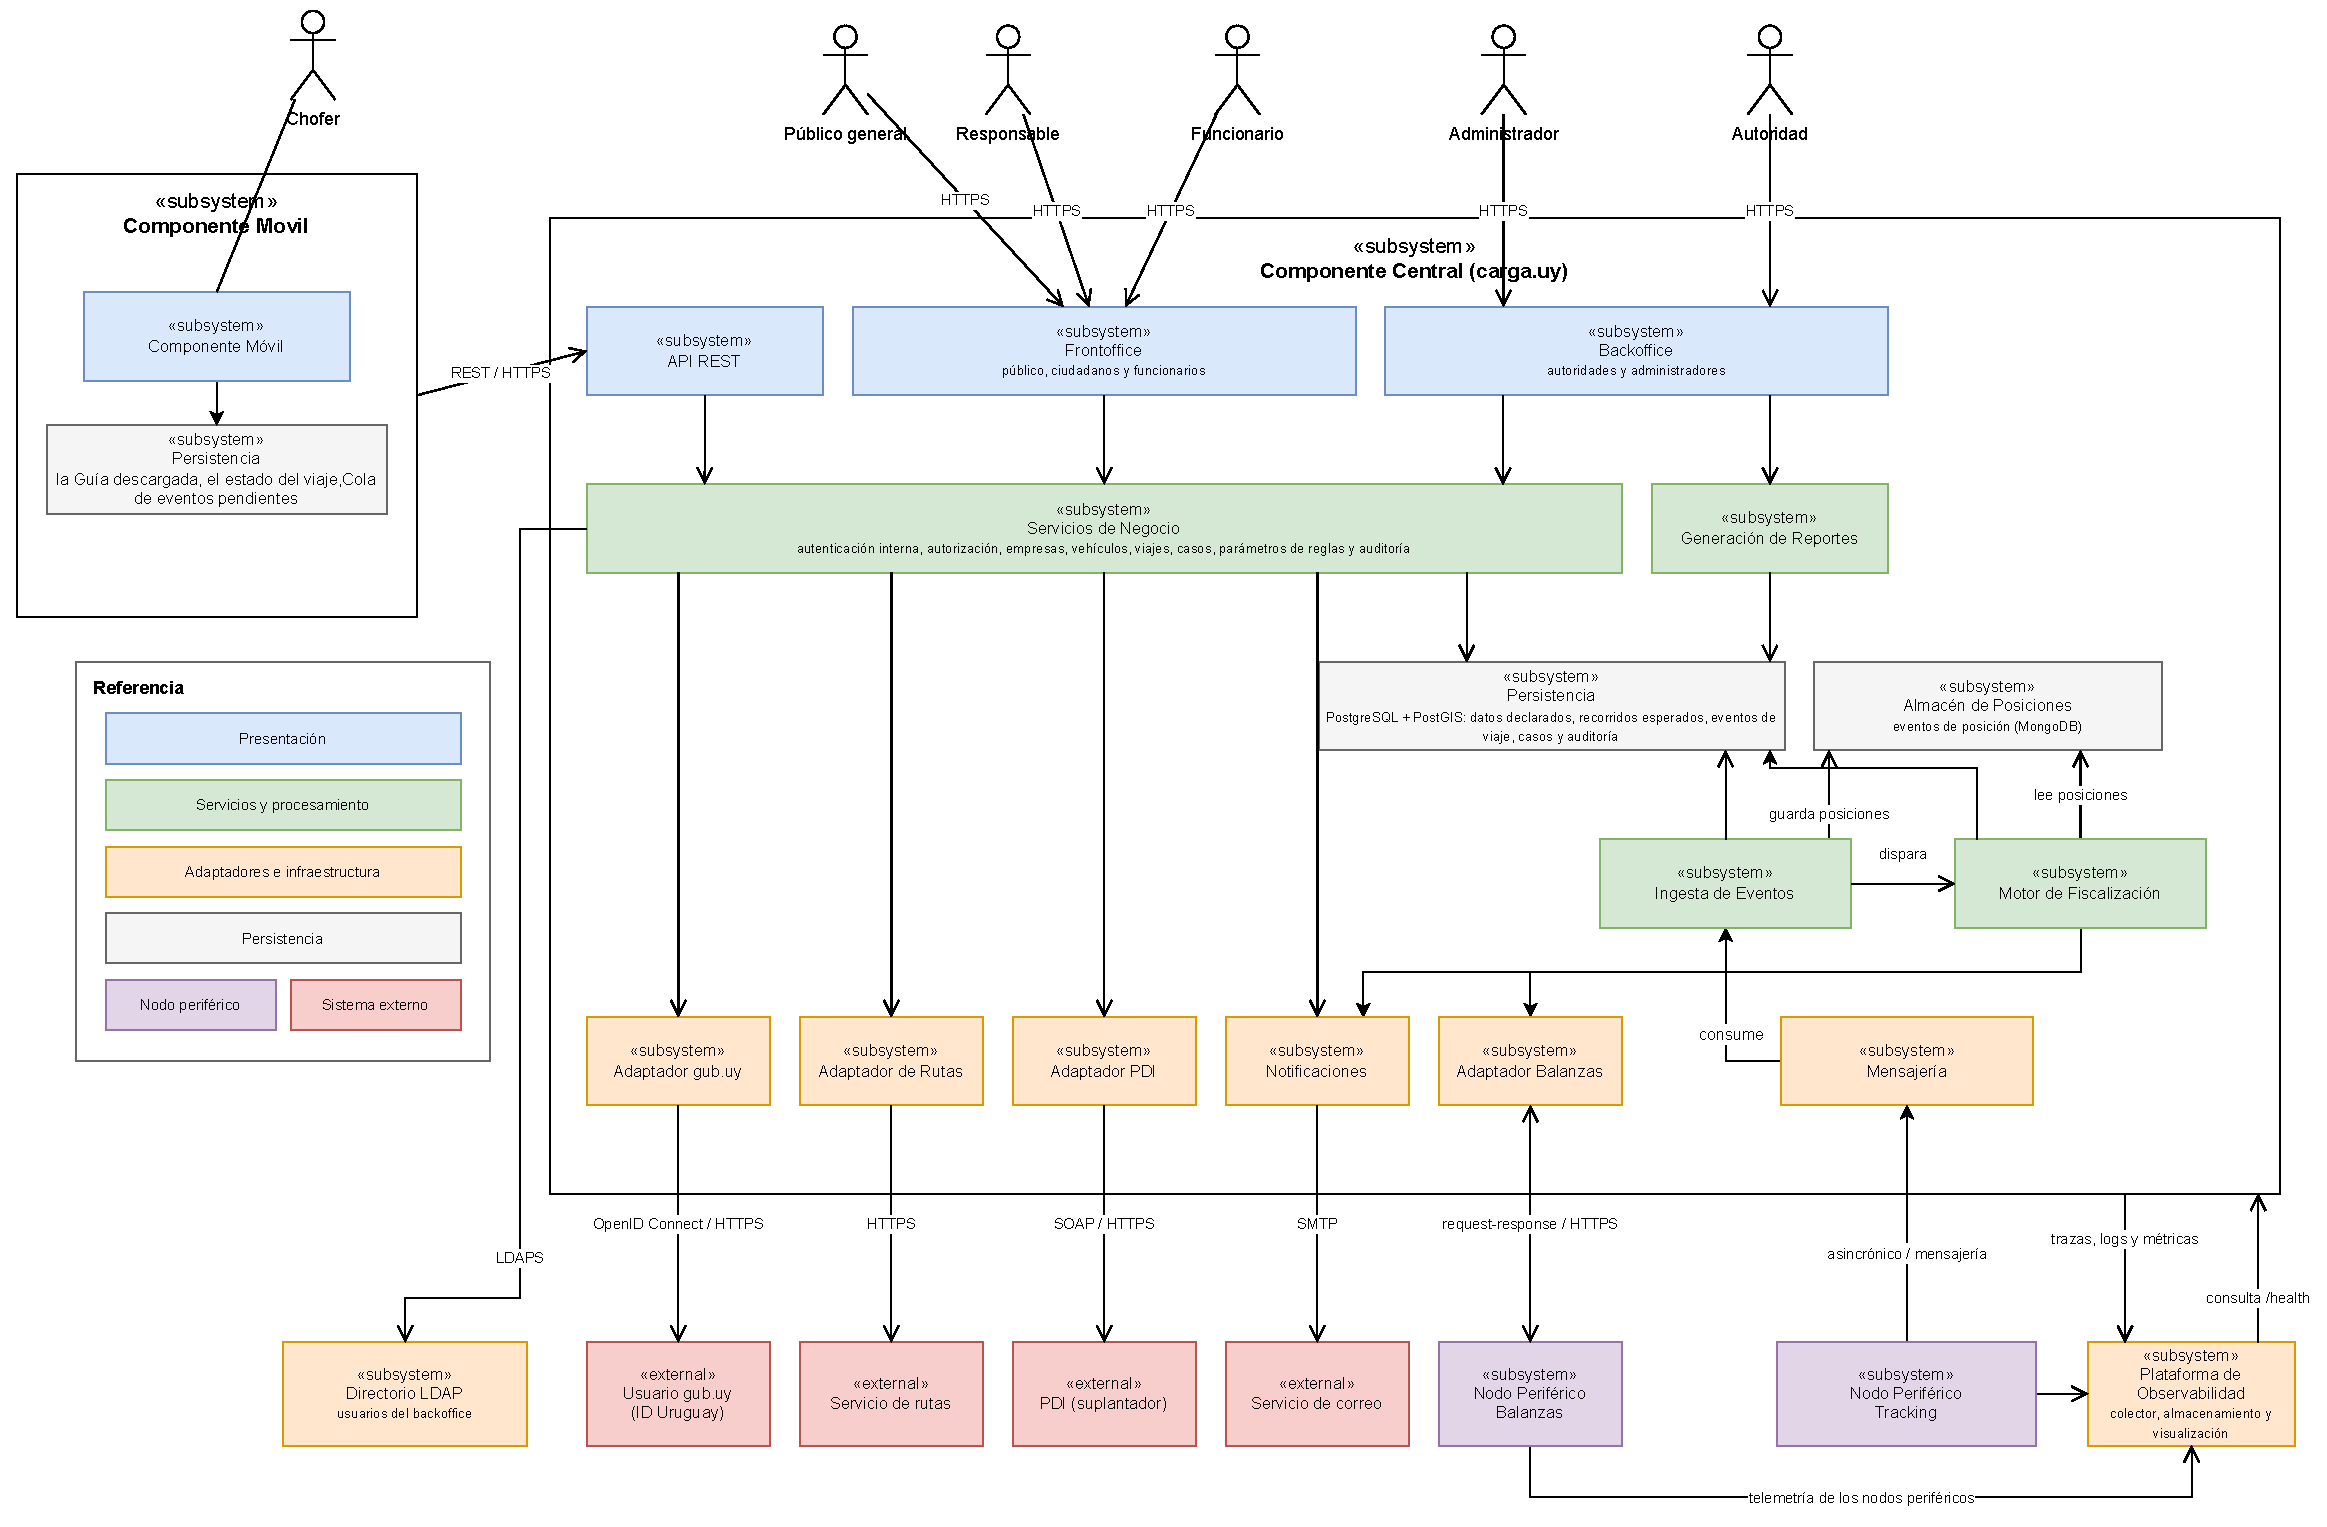
\includegraphics[width=\textwidth]{figures/vista-logica.pdf}
    \caption{Arquitectura general del sistema}
    \label{fig:vista_logica}
\end{figure}

\FloatBarrier

\subsection{Refinamiento 1: Ingesta de Eventos y nodos periféricos}\label{sec:refinamiento-ingesta}

Este refinamiento detalla los subsistemas Mensajería e Ingesta de Eventos, que realizan el CU-10, y el registro de nodos periféricos de los Servicios de Negocio, que realiza el CU-19. La Figura \ref{fig:refinamiento-ingesta} muestra sus componentes, con el clasificador \enquote{component}, y las dependencias entre ellos y con los demás subsistemas de la Figura \ref{fig:vista_logica}. La Tabla \ref{tab:refinamiento-ingesta} describe la responsabilidad de cada componente. Ambas corresponden a lo implementado; el Motor de Fiscalización figura como previsto.

\begin{figure}[H]
    \centering
    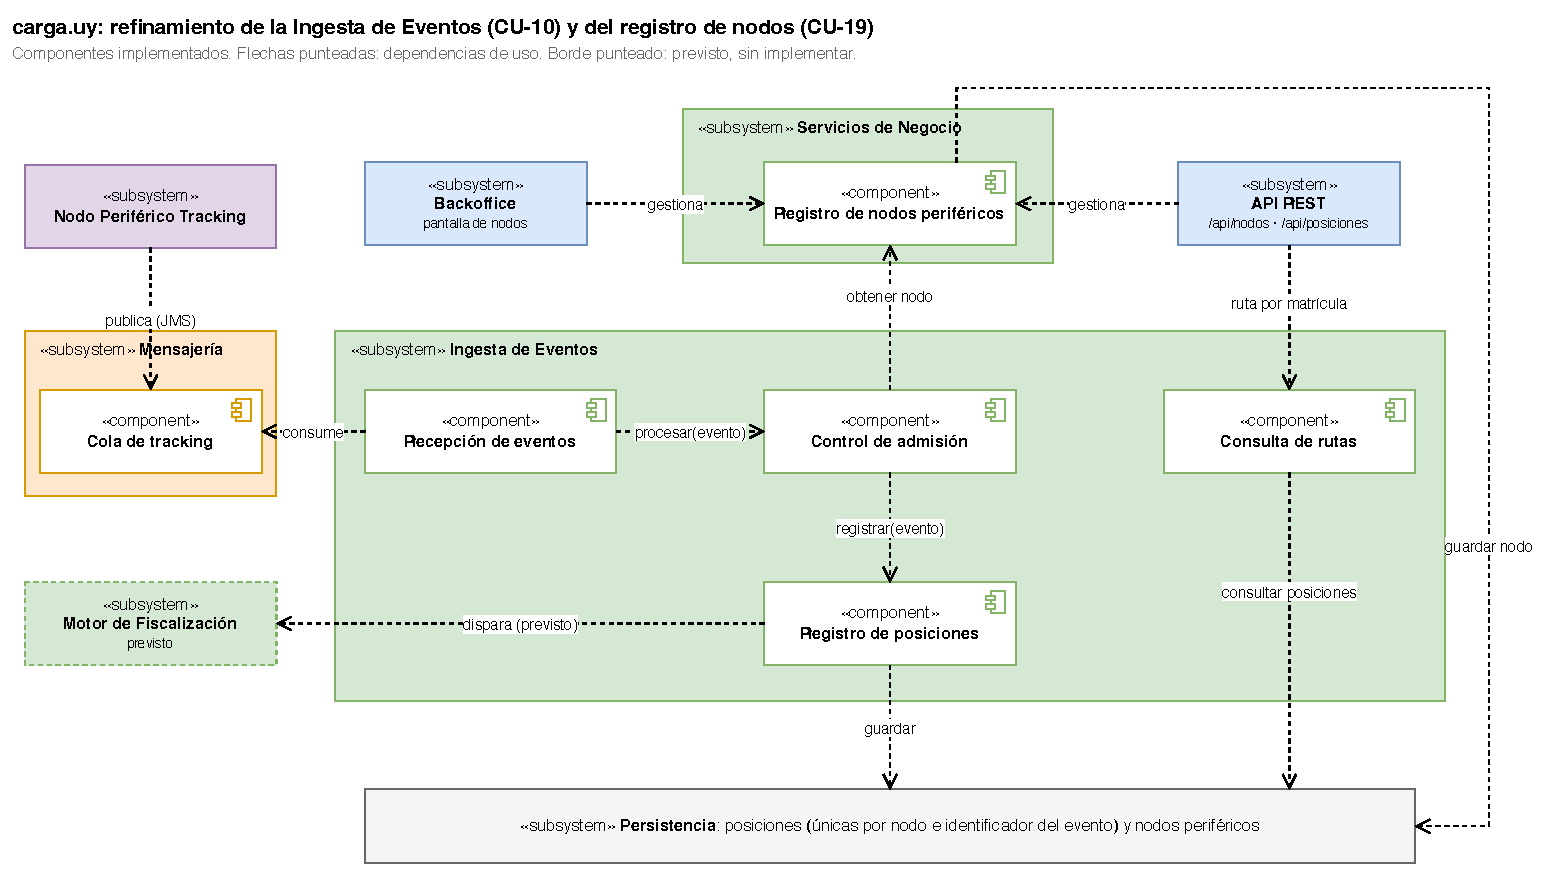
\includegraphics[width=\textwidth]{figures/refinamiento-ingesta.pdf}
    \caption{Vista Lógica, Refinamiento 1: Ingesta de Eventos y nodos periféricos}
    \label{fig:refinamiento-ingesta}
\end{figure}

\begin{table}[H]
    \small
    \centering
    \caption{Componentes de la ingesta de eventos y del registro de nodos}
    \label{tab:refinamiento-ingesta}
    \begin{tabular}{|p{3.6cm}|p{12.2cm}|}
        \hline
        \textbf{Componente} & \textbf{Responsabilidad} \\
        \hline
        Cola de tracking & Recibe los eventos de posición que publica el nodo periférico de tracking. Desacopla la recepción del procesamiento (R4). \\
        \hline
        Recepción de eventos & Consume la cola, interpreta cada evento y descarta los mensajes mal formados. Ante cualquier otra falla deja que el mecanismo de mensajería reentregue el evento. \\
        \hline
        Control de admisión & Acepta solo los eventos de un nodo de tracking registrado y habilitado, que es la precondición del CU-10. \\
        \hline
        Registro de posiciones & Asocia el evento al vehículo por su matrícula y lo almacena. Un evento repetido del mismo nodo choca contra una restricción de unicidad sobre el par (nodo, identificador del evento) y se descarta, lo que hace idempotente la ingesta (R6, AC15). \\
        \hline
        Consulta de rutas & Devuelve las posiciones de un vehículo ordenadas por su momento de generación y no por el orden de llegada (AC16). \\
        \hline
        Registro de nodos periféricos & Mantiene los nodos de balanzas y de tracking con su tipo, punto de acceso y estado. Todo nodo nuevo queda deshabilitado; cambiar su punto de acceso lo vuelve a deshabilitar; la baja es lógica (CU-19). \\
        \hline
    \end{tabular}
\end{table}

\pendiente{agregar los refinamientos de los demás subsistemas que el grupo considere necesarios, por ejemplo los Servicios de Negocio o el Motor de Fiscalización.}

\FloatBarrier

\subsection{Diagramas de Interacción}

En esta sección se incluyen diagramas de secuencia UML, a nivel de componentes, vinculados a los casos de uso críticos que se consideró necesario especificar con mayor detalle.

\subsubsection{CU-10 Ingerir y procesar eventos de tracking}\label{sec:interaccion-cu10}

La Figura \ref{fig:secuencia-cu10} muestra la interacción para el CU-10, de acuerdo con el refinamiento de la Sección \ref{sec:refinamiento-ingesta}. El nodo periférico de tracking publica el evento en la Mensajería, que lo entrega a la Ingesta de Eventos de forma asincrónica. Un mensaje mal formado se descarta sin reintento. La ingesta solo continúa si el evento proviene de un nodo de tracking registrado y habilitado; en ese caso obtiene el vehículo por su matrícula y registra el evento. Si el par (nodo, identificador del evento) ya estaba registrado, la restricción de unicidad lo rechaza y el evento se descarta como duplicado. Si es nuevo, se asocia al viaje que estaba en curso cuando se generó (Sección \ref{sec:cu-10}), se dispara el Motor de Fiscalización (Sección \ref{sec:interaccion-cu11}) y se actualizan las métricas. El orden de la ruta se reconstruye al consultarla, por el momento de generación de cada evento.

\begin{figure}[H]
    \centering
    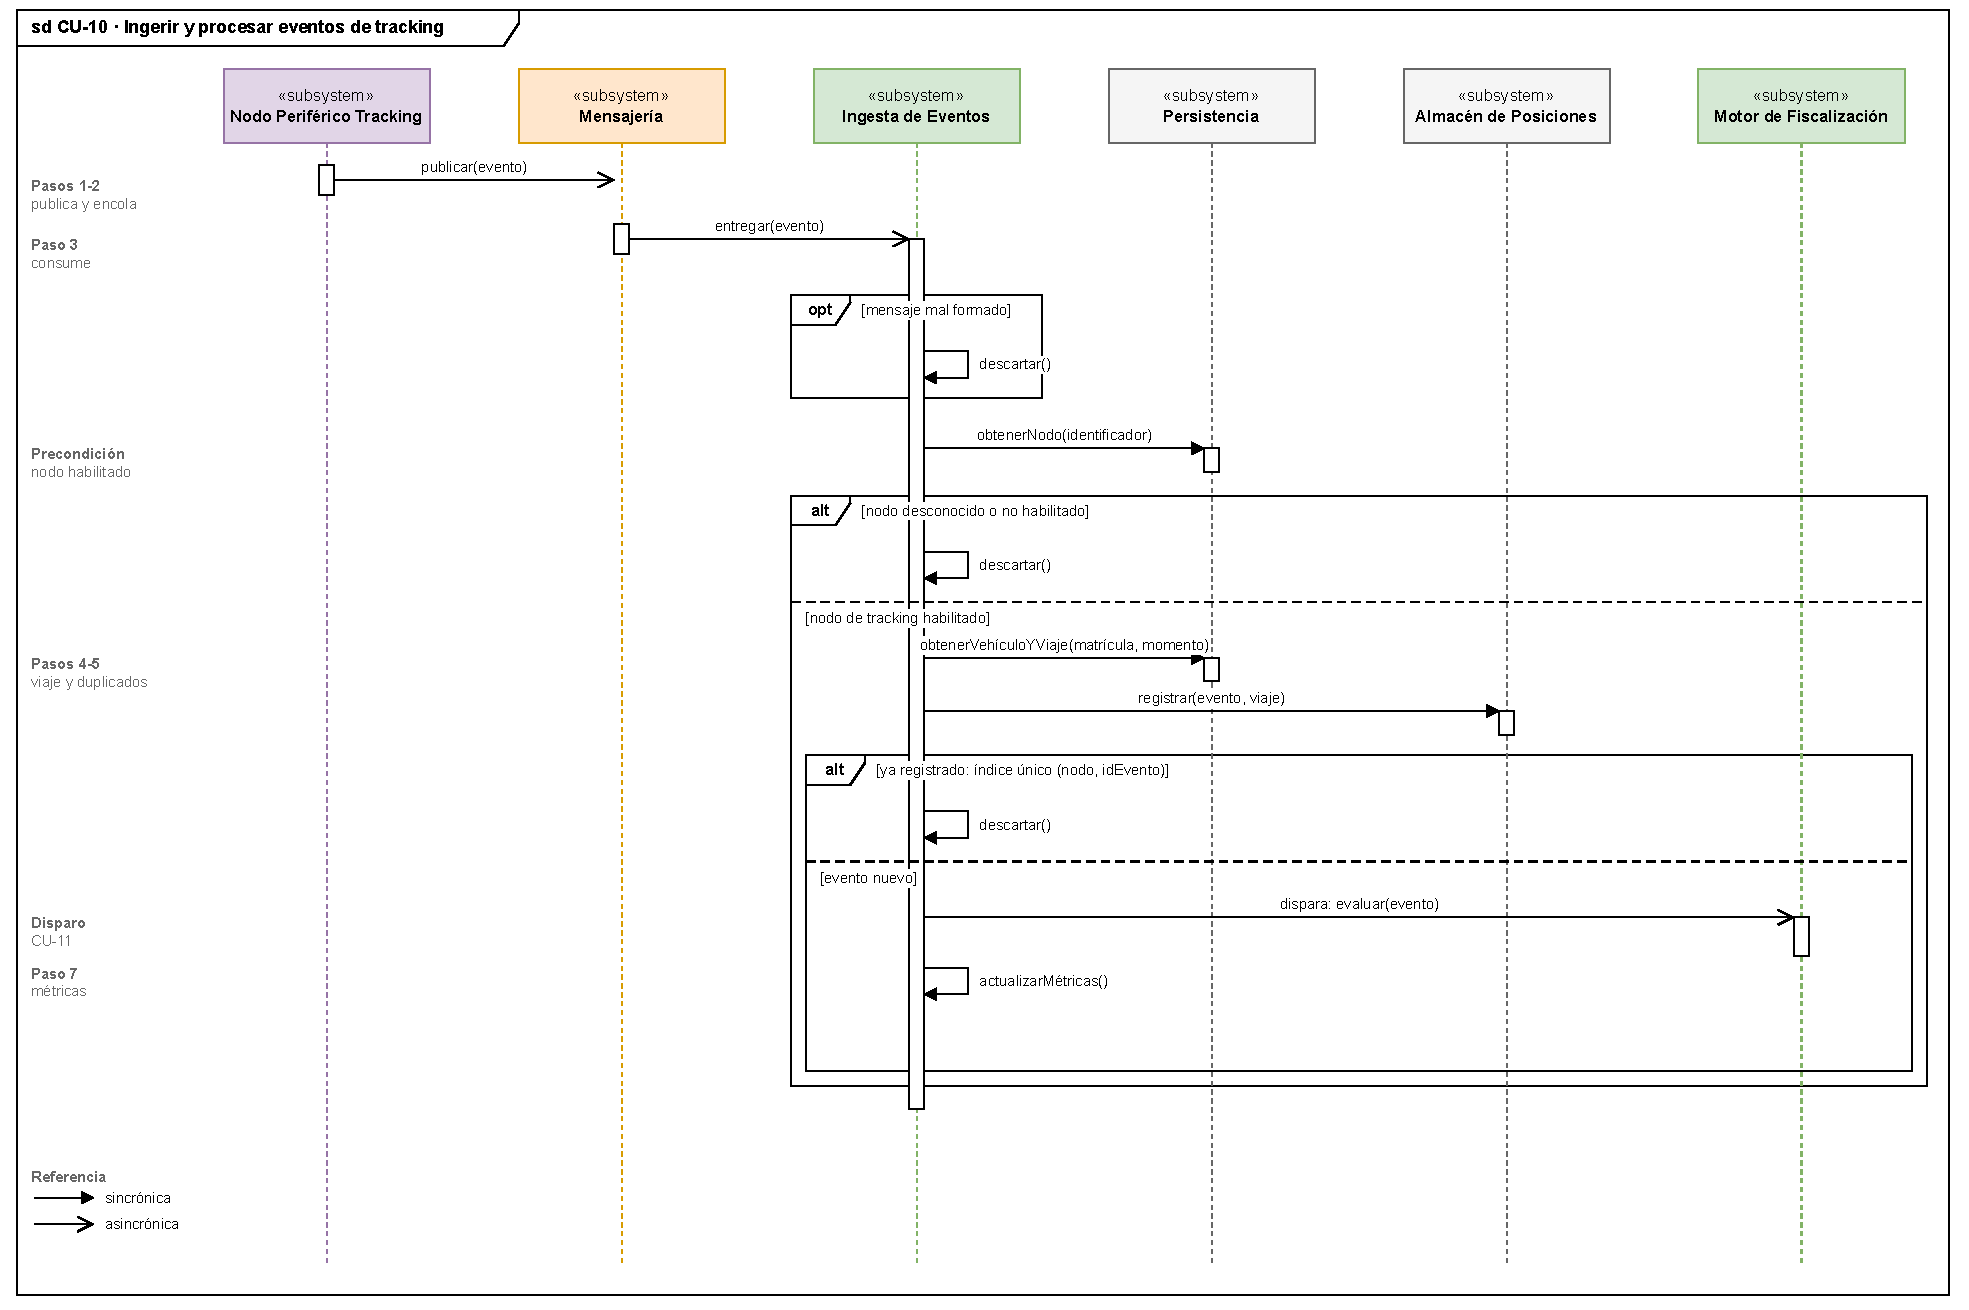
\includegraphics[width=\textwidth]{figures/secuencia-cu10.pdf}
    \caption{Diagrama de secuencia del CU-10}
    \label{fig:secuencia-cu10}
\end{figure}

\FloatBarrier

\subsubsection{CU-11 Detectar automáticamente un incumplimiento y generar el caso}\label{sec:interaccion-cu11}

La Figura \ref{fig:secuencia-cu11} muestra la interacción entre los componentes de la vista lógica para el CU-11. Comienza cuando la Ingesta de Eventos, al terminar el procesamiento del CU-10, dispara de forma asincrónica al Motor de Fiscalización. El fin de un viaje registrado desde el móvil (CU-09) dispara el mismo flujo. El motor evalúa las cuatro reglas de la Sección \ref{sec:vista-casos-de-uso}: exceso de carga, consultando los pesajes al nodo de Balanzas solo cuando el evento es el fin de un viaje (DA10); vigencia del Permiso y la ITV; viaje sin Guía; y desvío de ruta, contra el recorrido esperado y los umbrales parametrizados. Si detecta un incumplimiento, verifica que el hecho no haya generado otro caso; si no existe, crea el caso con su evidencia, notifica a la empresa, inicia el plazo de descargo y registra la creación en la pista de auditoría. Los pasos y las alternativas siguen la ficha del CU-11.

La notificación a la empresa es asincrónica: el motor le pide el aviso al subsistema de Notificaciones y continúa, para que una falla del correo no bloquee la creación del caso. El caso pasa a \emph{notificada}, y comienza el plazo de descargo, recién cuando el servidor de correo acepta el envío. Si el envío falla, Notificaciones lo reintenta y el caso permanece en \emph{detectada}, de modo que a la empresa no se le cuenta el plazo de un aviso que todavía no recibió. La creación del caso se registra en la pista de auditoría al final, como indica la ficha del CU-11.

\begin{figure}[H]
    \centering
    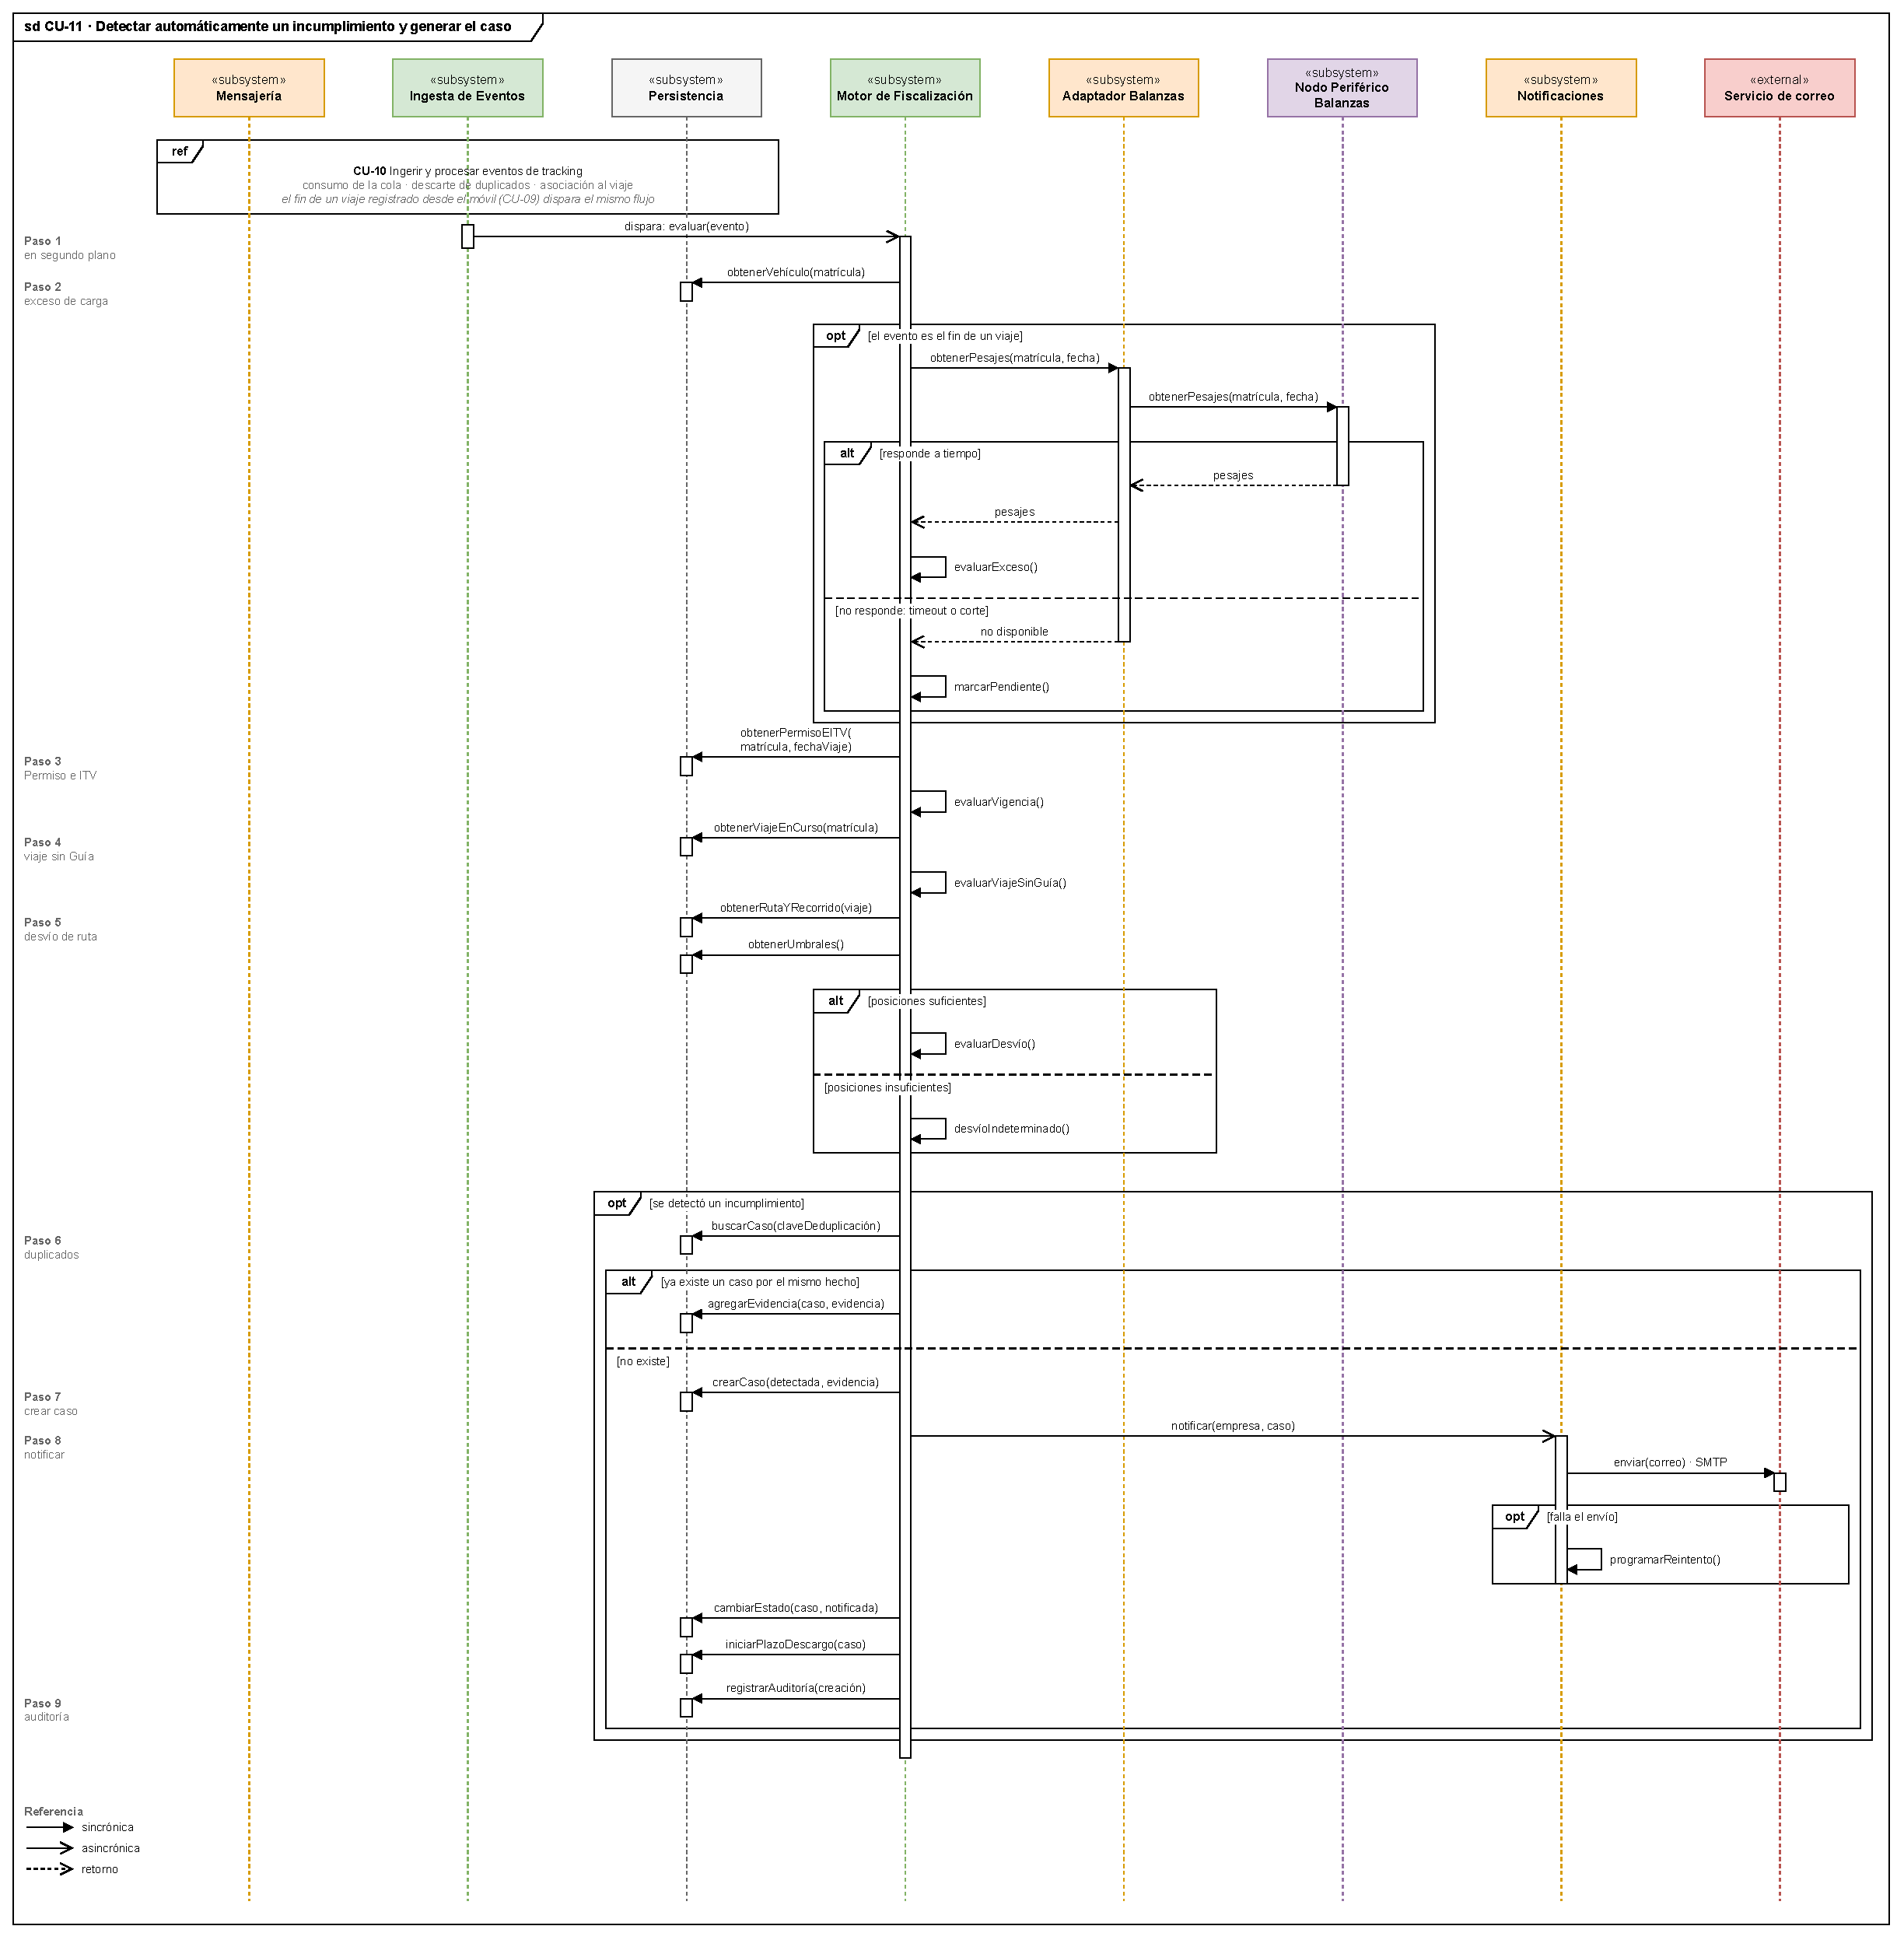
\includegraphics[width=\textwidth]{figures/secuencia-cu11.pdf}
    \caption{Diagrama de secuencia del CU-11}
    \label{fig:secuencia-cu11}
\end{figure}

\FloatBarrier

\section{Vista de Distribución}\label{sec:vista-de-distribucion}

En la vista de distribución o \textit{deployment} se plantean escenarios de distribución de los componentes en nodos, con las conexiones entre nodos y los componentes que corre cada uno. Para cada escenario interesa particularmente la descripción de los requerimientos no funcionales que lo justifican \cite{Perovich2003}.

Se utiliza el Diagrama de Deployment UML \cite{Ambysoft2018}. Los nodos físicos llevan el estereotipo \enquote{device}, los servidores y el navegador \enquote{executionEnvironment} y las plataformas en la nube \enquote{PaaS}. Dentro de cada nodo se indican los subsistemas de la Vista Lógica que corre, y cada conexión se rotula con su protocolo.

\begin{figure}[H]
    \centering
    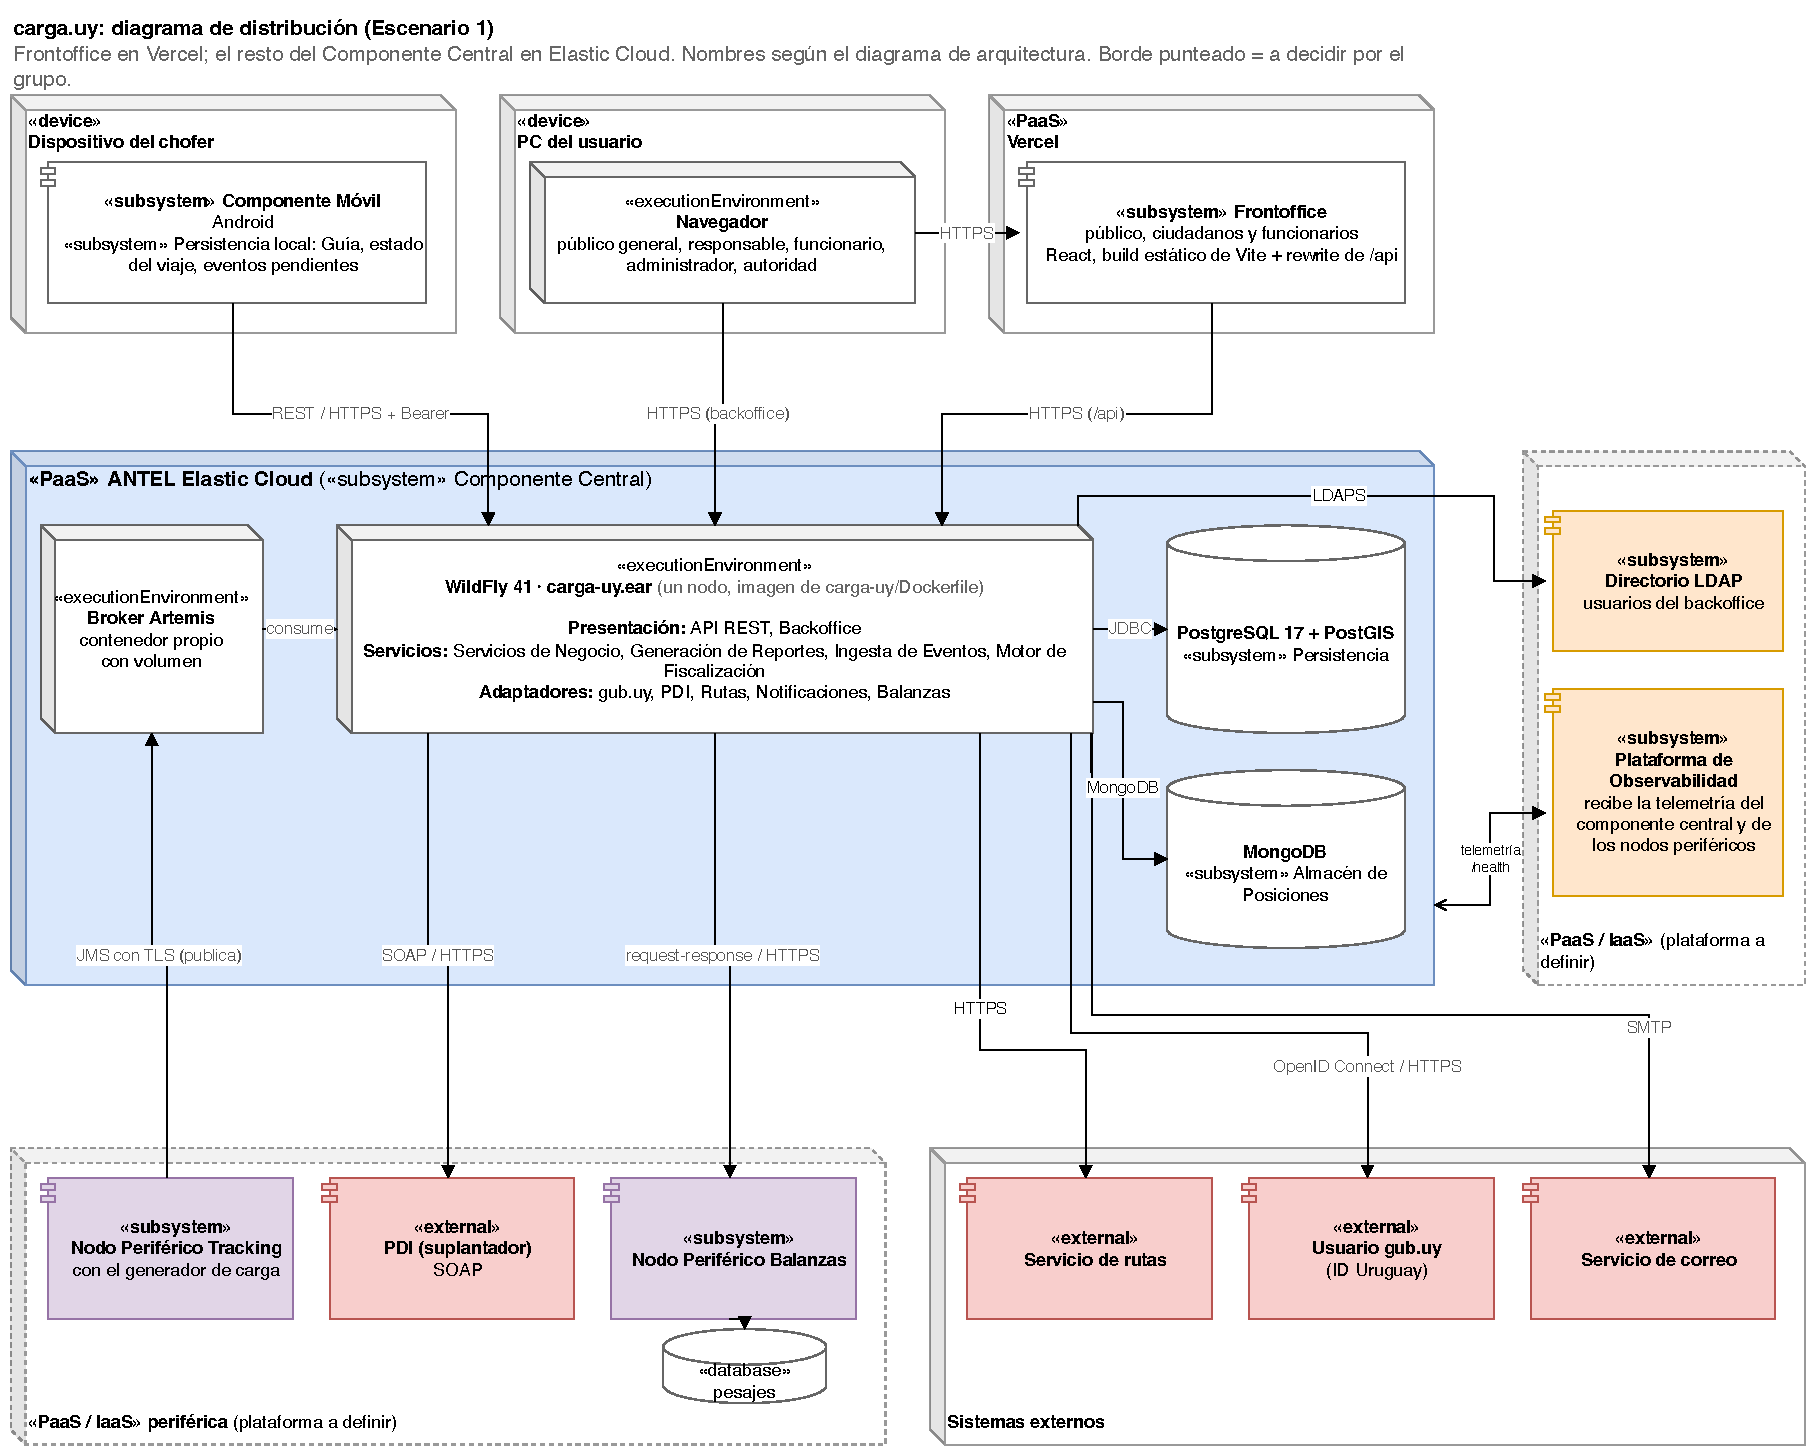
\includegraphics[width=\textwidth]{figures/vista-distribucion.pdf}
    \caption{Vista de Distribución, Escenario 1}
    \label{fig:vista_distrib}
\end{figure}

\subsection{Escenario 1: prototipo}

La Figura \ref{fig:vista_distrib} muestra la distribución prevista para el prototipo. Todas las conexiones entre entornos van por HTTPS (R8), salvo la del nodo de tracking con la mensajería, que se discute al final de esta sección.

\textbf{Dispositivo del chofer.} Corre el Componente Móvil (Android) con su persistencia local, que conserva la Guía, el estado del viaje y los eventos pendientes. Se comunica con el componente central mediante REST sobre HTTPS, con un token \textit{Bearer} (R2).

\textbf{PC del usuario.} El navegador accede al frontoffice y, para el backoffice, directamente al componente central.

\textbf{Vercel.} Sirve el frontoffice, construido en React como sitio estático, y redirige las llamadas a \texttt{/api} hacia el componente central.

\textbf{ANTEL Elastic Cloud (componente central).} Corre el servidor de aplicaciones WildFly con la aplicación empaquetada como EAR (presentación: API REST y backoffice; servicios: Servicios de Negocio, Generación de Reportes, Ingesta de Eventos y Motor de Fiscalización; adaptadores: gub.uy, PDI, notificaciones y balanzas), la base de datos PostgreSQL y la mensajería (R14).

\textbf{PaaS o IaaS periférica.} Corre los nodos periféricos de balanzas y de tracking, y el suplantador de la PDI (R15). El componente central consulta a balanzas en modalidad solicitud--respuesta (R3) y recibe los eventos de tracking a través de la mensajería (R4).

\textbf{Sistemas externos.} Usuario gub.uy (OpenID Connect) y el servicio de correo (SMTP).

\pendiente{describir los requerimientos no funcionales que justifican este escenario.}

\pendiente{confirmar con el tutor que los frontoffices pueden servirse desde Vercel: la letra ubica los frontoffices en el componente central y exige que el componente central corra en Elastic Cloud (R14).}

\pendiente{resolver la ubicación de la mensajería: el diagrama la muestra como un broker aparte, \enquote{a definir}, mientras que el grupo había decidido embeberla en el servidor de aplicaciones (DA02). Definir también cómo cumple R8 la conexión del nodo de tracking con la mensajería, porque los protocolos de los brokers no son HTTPS.}

\pendiente{agregar los componentes de observabilidad (colector de telemetría, trazas y métricas) y, si se adopta, la separación entre el generador de carga y el nodo de tracking.}

\subsection{Escenario 2}

\pendiente{definir si corresponde un segundo escenario, por ejemplo con varias instancias del servidor de aplicaciones detrás de un balanceador para verificar el escalado horizontal (AC07) en la prueba de performance.}

\section{Vista de Implementación}\label{sec:vista-de-implementacion}

La vista de implementación se centra en los componentes en tiempo de ejecución que forman el sistema (ejecutables, bibliotecas y \textit{frameworks}), que son la implementación de los componentes lógicos de la Sección \ref{sec:vista-logica}, y en las dependencias entre ellos.

\subsection{Componentes Ejecutables}

La Tabla \ref{tab:ejecutables} muestra los componentes ejecutables de la solución, la tecnología de cada uno y los subsistemas lógicos que implementan.

\begin{longtable}{|p{3.3cm}|p{5.4cm}|p{6.8cm}|}
    \caption{Componentes ejecutables}\label{tab:ejecutables}\\
    \hline
    \textbf{Componente} & \textbf{Tecnología} & \textbf{Subsistemas que implementa} \\
    \hline
    \endfirsthead
    \hline
    \textbf{Componente} & \textbf{Tecnología} & \textbf{Subsistemas que implementa} \\
    \hline
    \endhead
    \texttt{carga-uy.ear} & Jakarta EE 10 sobre WildFly 41, Java 24. Módulos \texttt{carga-uy-web} (JAX-RS y JSF), \texttt{carga-uy-ejb} (EJB) y \texttt{carga-uy-datos} (JPA con Hibernate). Sesiones con JWT mediante JJWT 0.13; cada request se autentica con un mecanismo de Jakarta Security que valida el JWT, y la autorización se declara con \texttt{@RolesAllowed} en los EJB. & API REST, Backoffice, Servicios de Negocio, Ingesta de Eventos, Adaptador gub.uy y acceso a la Persistencia. \\
    \hline
    Frontend web & React 19 con TypeScript, Tailwind CSS 4 y componentes shadcn/ui, construido con Vite 8. & Frontoffice de Ciudadanos y Frontoffice de Funcionarios. \\
    \hline
    Aplicación móvil & Android (\textit{compileSdk} 37, \textit{minSdk} 26), Kotlin 2.4, Jetpack Compose y Room 2.8 para la persistencia local. & Componente Móvil y su persistencia local. \\
    \hline
    Base de datos & PostgreSQL 17, con el controlador JDBC 42.7.7. & Persistencia. \\
    \hline
    Broker de mensajería & ActiveMQ Artemis embebido en WildFly, con la cola \texttt{queue\_tracking}. & Mensajería. \\
    \hline
    Nodo de tracking simulado & Java 17 con el cliente JMS remoto de WildFly. & Nodo Periférico Tracking. \\
    \hline
\end{longtable}

Todavía no tienen implementación la Generación de Reportes, el Motor de Fiscalización, los adaptadores de la PDI, de notificaciones y de balanzas, el nodo periférico de balanzas y el suplantador de la PDI.

\pendiente{describir los pros y los contras de las tecnologías elegidas y las habilidades necesarias para el proyecto, como pide la plantilla para esta vista.}

\subsection{Dependencias entre Componentes}

La Figura \ref{fig:vista_impl} muestra, con un diagrama de deployment UML \cite{Ambysoft2018}, los artefactos de la Tabla \ref{tab:ejecutables}, el entorno de ejecución en que corre cada uno y las dependencias entre ellos, de acuerdo con el estado actual del repositorio. La distribución prevista para producción se describe en la Sección \ref{sec:vista-de-distribucion}.

\begin{figure}[H]
    \centering
    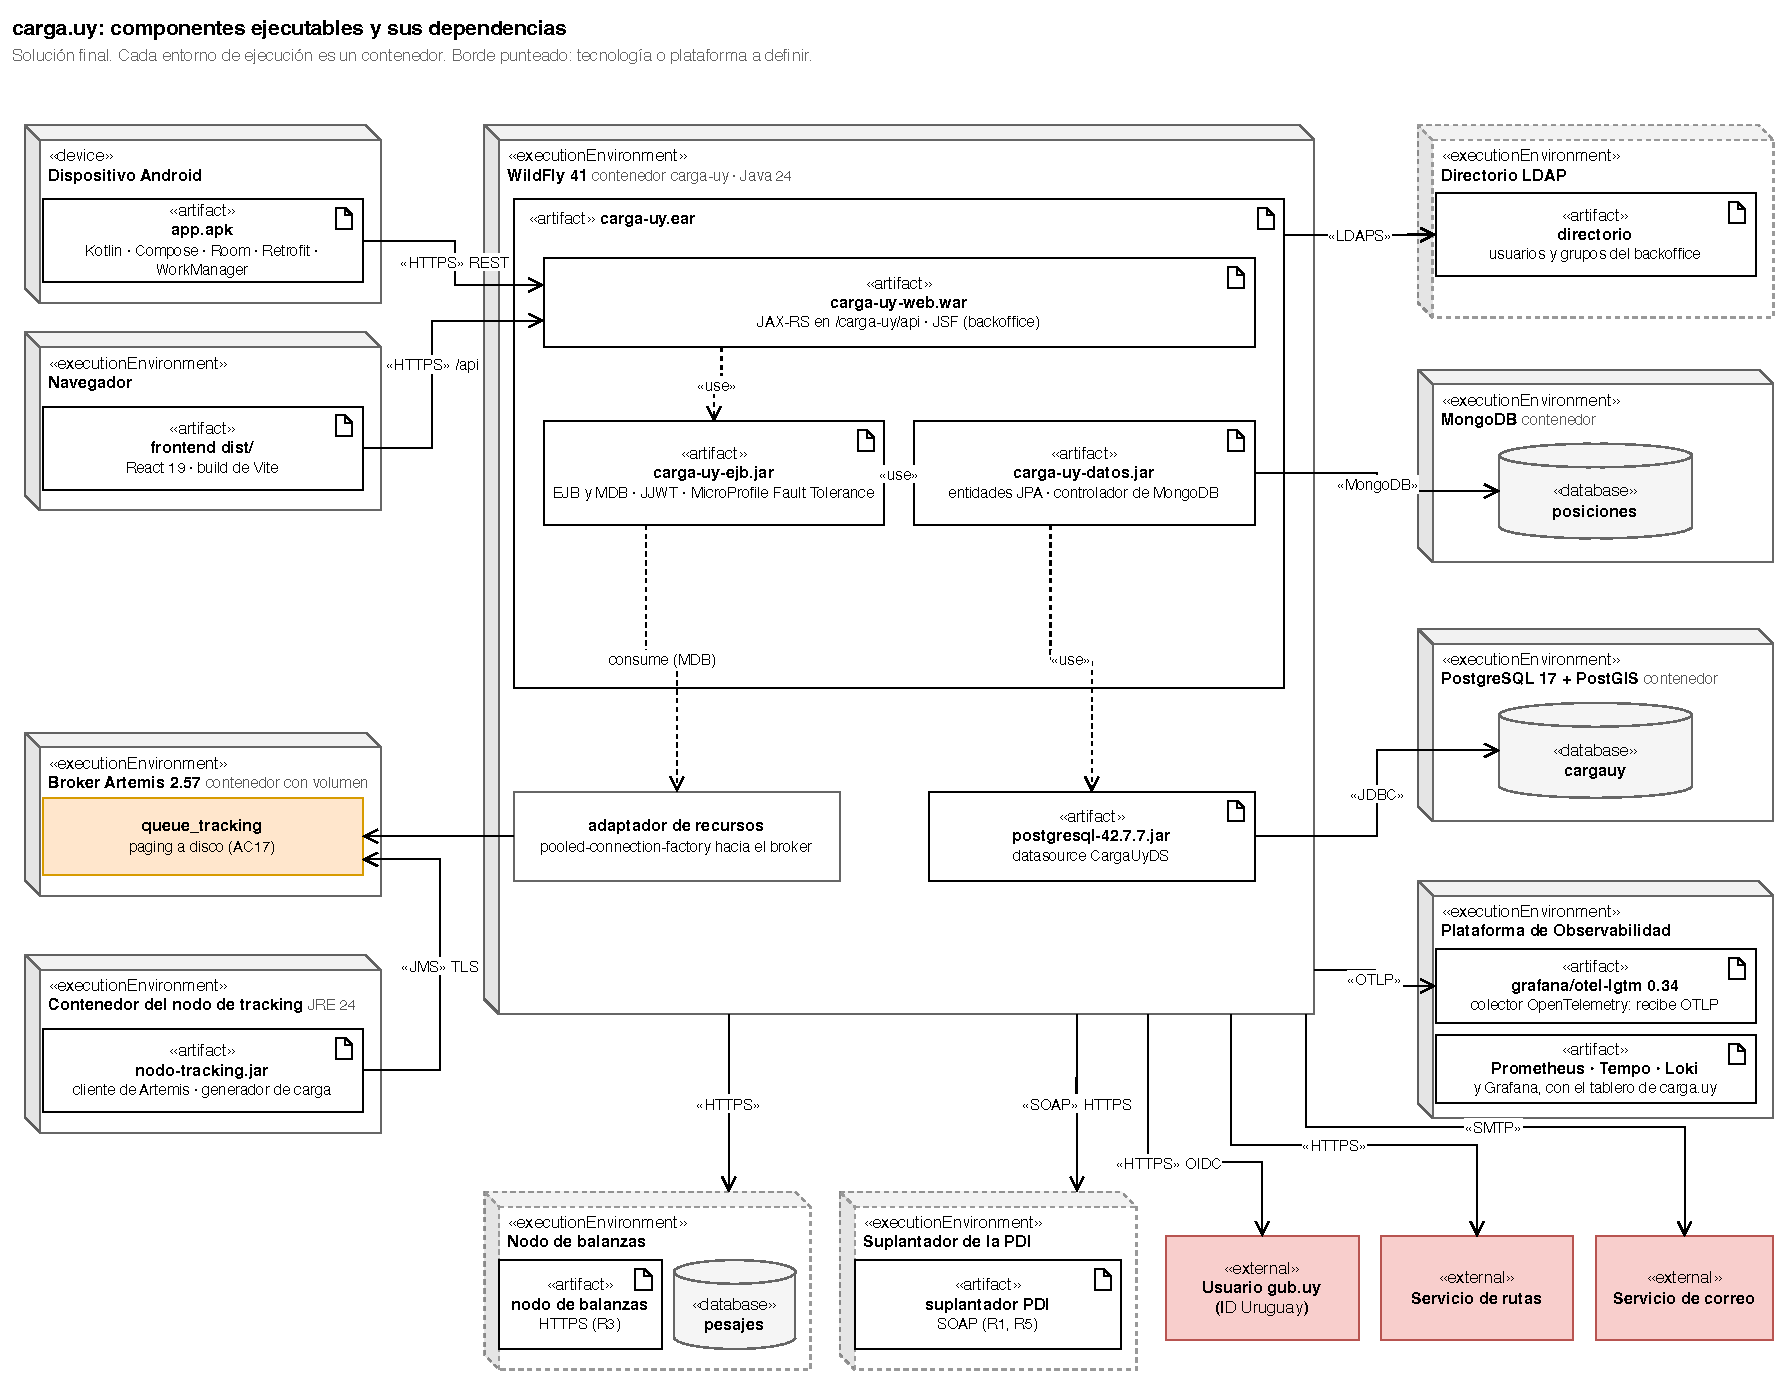
\includegraphics[width=0.9\textwidth]{figures/implementacion.pdf}
    \caption{Vista de Implementación}
    \label{fig:vista_impl}
\end{figure}

\begin{itemize}
    \item Dentro del EAR, \texttt{carga-uy-web} depende de \texttt{carga-uy-ejb}, y este de \texttt{carga-uy-datos}.
    \item El frontend web y la aplicación móvil consumen la API REST del EAR. En desarrollo, el frontend redirige las llamadas a \texttt{/api} hacia el componente central.
    \item El nodo de tracking publica en la cola \texttt{queue\_tracking}, a la que accede como cliente JMS remoto a través del puerto web de WildFly.
    \item El EAR accede a PostgreSQL mediante el \textit{datasource} \texttt{CargaUyDS} y a Usuario gub.uy mediante OpenID Connect.
\end{itemize}

\subsection{Empaquetado}

El componente central se distribuye como una imagen de contenedor construida en dos etapas: la primera compila el proyecto con Maven y la segunda configura WildFly 41 con el controlador de PostgreSQL, el \textit{datasource} y las colas JMS, y despliega el EAR. Un archivo de Docker Compose levanta la base de datos y el componente central. La configuración sensible (credenciales de gub.uy y secreto de los tokens de sesión) se pasa por variables de entorno desde un archivo \texttt{.env} que no se sube al repositorio.

\pendiente{completar R13: el frontend y el nodo de tracking todavía no están contenerizados, así que el entorno completo no se levanta con un único comando. Además, el Dockerfile crea un usuario de WildFly con credenciales escritas en el repositorio (R11).}

\subsection{Integración Continua}

Ante cada modificación, el pipeline del repositorio del grupo en el GitLab de FING debe ejecutar como mínimo la compilación de todos los componentes, las pruebas automatizadas, el análisis estático de calidad del código y la construcción de los artefactos o imágenes de contenedor, y debe estar en estado exitoso al momento de la entrega final (R16, R17).

Hoy el repositorio está en GitHub y tiene un pipeline de GitHub Actions que, en cada \textit{pull request} y en cada cambio en la rama principal, compila el backend, corre las pruebas de \texttt{carga-uy}, \texttt{carga-uy-client} y \texttt{nodo-tracking}, y ejecuta el lint y la construcción del frontend.

\pendiente{migrar el repositorio y el pipeline al GitLab de FING, y agregar el análisis estático de calidad (por ejemplo, SonarQube) y la construcción de las imágenes de contenedor.}

\section{Vista de Decisiones de Arquitectura}\label{sec:vista-de-decisiones-de-arquitectura}

La Vista de Decisiones de Arquitectura presenta y describe las principales decisiones de arquitectura tomadas \cite{VanHeesch2012}\cite{Kruchten2009}. Para cada decisión se especifican los campos de la plantilla: identificador, nombre, categorías, problema, alternativas, decisión, justificación y decisiones relacionadas.


\begin{table}[H]
    \small
    \centering
    \caption{DA01: Arquitectura en capas del componente central}
    \label{tab:da01}
    \begin{tabular}{|p{4.1cm}|p{11.7cm}|}
        \hline
            \textbf{Identificador} & DA01 \\
        \hline
            \textbf{Nombre} & Arquitectura en capas del componente central \\
        \hline
            \textbf{Categorías} & Componente central; mantenibilidad. \\
        \hline
            \textbf{Problema} & El componente central concentra la presentación para cuatro tipos de usuarios y la API del componente móvil, la lógica de negocio y de fiscalización, la persistencia y la integración con varios sistemas externos y nodos periféricos. \\
        \hline
            \textbf{Alternativas} & \pendiente{completar las alternativas consideradas.} \\
        \hline
            \textbf{Decisión} & Organizar el componente central en cuatro capas: presentación (API REST, frontoffice y backoffice), servicios y procesamiento (Servicios de Negocio, Generación de Reportes, Ingesta de Eventos y Motor de Fiscalización), persistencia, y adaptadores e infraestructura, que aíslan cada integración externa (Figura \ref{fig:vista_logica}). \\
        \hline
            \textbf{Justificación} & \pendiente{completar la justificación.} \\
        \hline
            \textbf{Decisiones Relacionadas} & DA02, DA05 \\
        \hline
    \end{tabular}
\end{table}

\begin{table}[H]
    \small
    \centering
    \caption{DA02: Broker de mensajería en su propio contenedor}
    \label{tab:da02}
    \begin{tabular}{|p{4.1cm}|p{11.7cm}|}
        \hline
            \textbf{Identificador} & DA02 \\
        \hline
            \textbf{Nombre} & Broker de mensajería en su propio contenedor \\
        \hline
            \textbf{Categorías} & Mensajería; integración con tracking; R4, R8; AC07, AC08, AC15, AC17. \\
        \hline
            \textbf{Problema} & La recepción de los eventos de tracking debe estar desacoplada de su procesamiento mediante un mecanismo de mensajería asincrónica (R4). La letra pide justificar la tecnología elegida, la estrategia de particionamiento o distribución de los mensajes y la política de entrega. \\
        \hline
            \textbf{Alternativas} & \pendiente{completar las alternativas consideradas.} \\
        \hline
            \textbf{Decisión} & Usar Apache Artemis (Jakarta Messaging) como broker en su propio contenedor, separado de WildFly y con los mensajes en un volumen. Los nodos de tracking publican en la cola \texttt{queue\_tracking} conectándose directo al broker con TLS (R8), cada uno con un usuario que solo puede publicar en esa cola. Todas las instancias del componente central consumen la misma cola, mediante el componente de recepción (Sección \ref{sec:refinamiento-ingesta}), y compiten por sus mensajes; el orden de la ruta se reconstruye por el momento de generación de cada posición (AC16) y los duplicados se descartan en la ingesta (DA07). La entrega es al menos una vez: un mensaje se borra de la cola cuando se confirma la transacción que lo procesó, y si el procesamiento falla, el broker lo vuelve a entregar. Si el procesamiento falla, la reentrega espera cada vez más (1~s, 2~s, 4~s\ldots{} hasta un minuto) y se hacen hasta 20 entregas: el componente central puede estar unos 14 minutos sin poder procesar sin perder posiciones. Recién entonces el mensaje pasa a la cola de mensajes muertos, que el tablero de la Plataforma de Observabilidad muestra y desde la que se reprocesa con la consola del broker; reprocesar es seguro porque la ingesta descarta los duplicados (DA07). \\
        \hline
            \textbf{Justificación} & \pendiente{completar la justificación.} \\
        \hline
            \textbf{Decisiones Relacionadas} & DA01, DA07 \\
        \hline
    \end{tabular}
\end{table}

\begin{table}[H]
    \small
    \centering
    \caption{DA03: Sesión sin estado en el servidor}
    \label{tab:da03}
    \begin{tabular}{|p{4.1cm}|p{11.7cm}|}
        \hline
            \textbf{Identificador} & DA03 \\
        \hline
            \textbf{Nombre} & Sesión sin estado en el servidor \\
        \hline
            \textbf{Categorías} & Seguridad; escalabilidad; AC07; CU-01. \\
        \hline
            \textbf{Problema} & El componente central debe escalar horizontalmente sin guardar estado local en las instancias (AC07). El ingreso con Usuario gub.uy necesita conservar \texttt{state}, \texttt{nonce} y \texttt{code\_challenge} entre el inicio del ingreso y el \textit{callback}. \\
        \hline
            \textbf{Alternativas} & Mantener ese estado en la \texttt{HttpSession} de la instancia y firmar el JWT de sesión con código propio, que fue la implementación inicial. \\
        \hline
            \textbf{Decisión} & La sesión es un JWT firmado (HS256) con la biblioteca JJWT, que viaja en una cookie \textit{HttpOnly} en la web y como token \textit{Bearer} en el móvil. El estado del ingreso con gub.uy viaja en una cookie firmada en lugar de quedar en la \texttt{HttpSession}. El secreto se configura por entorno y debe tener al menos 32 bytes. El JWT se emite también tras el ingreso al backoffice, que valida las credenciales contra el directorio LDAP. \\
        \hline
            \textbf{Justificación} & Hace la autenticación independiente de la instancia y saca la criptografía propia del código: el \textit{callback} de gub.uy puede llegar a cualquier instancia del componente central. \\
        \hline
            \textbf{Decisiones Relacionadas} & DA04, DA09 \\
        \hline
    \end{tabular}
\end{table}

\begin{table}[H]
    \small
    \centering
    \caption{DA04: Ingreso desde el móvil con \textit{authorization code} y PKCE}
    \label{tab:da04}
    \begin{tabular}{|p{4.1cm}|p{11.7cm}|}
        \hline
            \textbf{Identificador} & DA04 \\
        \hline
            \textbf{Nombre} & Ingreso desde el móvil con \textit{authorization code} y PKCE \\
        \hline
            \textbf{Categorías} & Seguridad; componente móvil; CU-01. \\
        \hline
            \textbf{Problema} & La aplicación móvil debe autenticar al chofer mediante Usuario gub.uy (CU-01) y obtener un token para llamar a la API REST (R2). \\
        \hline
            \textbf{Alternativas} & \pendiente{completar las alternativas consideradas.} \\
        \hline
            \textbf{Decisión} & La aplicación abre el ingreso en el navegador con un \texttt{code\_challenge}, recibe un código de un solo uso por el esquema \texttt{cargauy://ingreso} y lo canjea, junto con el \texttt{code\_verifier}, por el token de sesión. En Android, el ingreso se abre con Custom Tabs. \\
        \hline
            \textbf{Justificación} & \pendiente{completar la justificación.} \\
        \hline
            \textbf{Decisiones Relacionadas} & DA03 \\
        \hline
    \end{tabular}
\end{table}

\begin{table}[H]
    \small
    \centering
    \caption{DA05: Tecnologías de presentación y ubicación del frontoffice}
    \label{tab:da05}
    \begin{tabular}{|p{4.1cm}|p{11.7cm}|}
        \hline
            \textbf{Identificador} & DA05 \\
        \hline
            \textbf{Nombre} & Tecnologías de presentación y ubicación del frontoffice \\
        \hline
            \textbf{Categorías} & Presentación; distribución; R14. \\
        \hline
            \textbf{Problema} & La plataforma tiene un frontoffice para ciudadanos, otro para funcionarios y un backoffice para autoridades y administradores, todos web. \\
        \hline
            \textbf{Alternativas} & \pendiente{completar las alternativas consideradas.} \\
        \hline
            \textbf{Decisión} & Backoffice en JSF dentro del componente central; frontoffice en React, servido como sitio estático desde Vercel (Figura \ref{fig:vista_distrib}). \\
        \hline
            \textbf{Justificación} & \pendiente{completar la justificación.} \\
        \hline
            \textbf{Decisiones Relacionadas} & DA01 \\
        \hline
    \end{tabular}
\end{table}

\begin{table}[H]
    \small
    \centering
    \caption{DA06: Componente móvil nativo para Android}
    \label{tab:da06}
    \begin{tabular}{|p{4.1cm}|p{11.7cm}|}
        \hline
            \textbf{Identificador} & DA06 \\
        \hline
            \textbf{Nombre} & Componente móvil nativo para Android \\
        \hline
            \textbf{Categorías} & Componente móvil; AC18, AC19, AC20. \\
        \hline
            \textbf{Problema} & El chofer debe poder consultar la Guía y registrar los eventos del viaje sin conectividad, y la sincronización posterior debe ser idempotente. \\
        \hline
            \textbf{Alternativas} & \pendiente{completar las alternativas consideradas.} \\
        \hline
            \textbf{Decisión} & Aplicación nativa para Android en Kotlin con Jetpack Compose, persistencia local con Room y un identificador UUID generado en el dispositivo para cada evento pendiente. La sincronización corre en segundo plano con WorkManager, que espera a tener conexión y reintenta con esperas crecientes, y las llamadas a la API REST usan Retrofit con OkHttp. \\
        \hline
            \textbf{Justificación} & \pendiente{completar la justificación.} \\
        \hline
            \textbf{Decisiones Relacionadas} & DA04 \\
        \hline
    \end{tabular}
\end{table}

\begin{table}[H]
    \small
    \centering
    \caption{DA07: Posiciones en MongoDB con idempotencia por índice único}
    \label{tab:da07}
    \begin{tabular}{|p{4.1cm}|p{11.7cm}|}
        \hline
            \textbf{Identificador} & DA07 \\
        \hline
            \textbf{Nombre} & Posiciones en MongoDB con idempotencia por índice único \\
        \hline
            \textbf{Categorías} & Ingesta de eventos; opcional 10; R6; AC08, AC15, AC16. \\
        \hline
            \textbf{Problema} & Las posiciones son el dato de mayor volumen y solo se agregan. Además, un mismo evento de tracking puede recibirse más de una vez (reentregas del broker o reenvíos del nodo) y la cola tiene varios consumidores en paralelo. Un evento duplicado no debe alterar el estado del viaje ni generar casos adicionales. \\
        \hline
            \textbf{Alternativas} & Guardar las posiciones en PostgreSQL con una restricción de unicidad; usar una colección de series temporales de MongoDB. \\
        \hline
            \textbf{Decisión} & Guardar las posiciones en una colección normal de MongoDB, con un índice único sobre el par (nodo, identificador del evento) e índices por viaje y por matrícula con el momento de generación. Un evento que viola el índice único se descarta como duplicado. Como MongoDB no participa de la transacción del mensaje, cada posición se guarda sin procesar y se marca como procesada cuando se confirma esa transacción. Si llega de nuevo una posición que quedó sin procesar, porque un intento anterior falló después de guardarla, no se guarda otra vez pero se completan los pasos que siguen al guardado; si ya estaba procesada, se descarta. Las posiciones referencian el vehículo, el viaje y el nodo por su identificador, sin claves foráneas. \\
        \hline
            \textbf{Justificación} & Las posiciones son el dato que más crece en la plataforma, y guardarlas aparte evita que degraden a PostgreSQL. Se usa una colección normal de MongoDB y no una de series temporales, porque estas no admiten índices únicos para descartar duplicados ni permiten modificar una posición después para asociarla a su viaje. Si una posición llega de nuevo, el índice único la identifica como duplicada y no se guarda dos veces. \\
        \hline
            \textbf{Decisiones Relacionadas} & DA02, DA08 \\
        \hline
    \end{tabular}
\end{table}

\begin{table}[H]
    \small
    \centering
    \caption{DA08: Registro de nodos periféricos con estados}
    \label{tab:da08}
    \begin{tabular}{|p{4.1cm}|p{11.7cm}|}
        \hline
            \textbf{Identificador} & DA08 \\
        \hline
            \textbf{Nombre} & Registro de nodos periféricos con estados \\
        \hline
            \textbf{Categorías} & Servicios de negocio; CU-19; CU-10. \\
        \hline
            \textbf{Problema} & Los administradores deben poder gestionar los nodos periféricos (CU-19), y la ingesta de tracking solo debe aceptar eventos de un nodo registrado y habilitado, que es la precondición del CU-10. \\
        \hline
            \textbf{Alternativas} & \pendiente{completar las alternativas consideradas.} \\
        \hline
            \textbf{Decisión} & Un registro de nodos con tipo (balanzas o tracking), punto de acceso y estado (deshabilitado, habilitado o baja). Todo nodo nuevo arranca deshabilitado, cambiar el punto de acceso lo vuelve a deshabilitar y la baja es lógica. \\
        \hline
            \textbf{Justificación} & \pendiente{completar la justificación.} \\
        \hline
            \textbf{Decisiones Relacionadas} & DA07 \\
        \hline
    \end{tabular}
\end{table}

\begin{table}[H]
    \small
    \centering
    \caption{DA09: Autorización declarativa en la capa de servicios}
    \label{tab:da09}
    \begin{tabular}{|p{4.1cm}|p{11.7cm}|}
        \hline
            \textbf{Identificador} & DA09 \\
        \hline
            \textbf{Nombre} & Autorización declarativa en la capa de servicios \\
        \hline
            \textbf{Categorías} & Seguridad; servicios de negocio; R9; AC03. \\
        \hline
            \textbf{Problema} & La autorización debe aplicarse en la capa de servicios y no solo en la interfaz de usuario (R9). Además, un responsable o un chofer solo debe acceder a los datos de su propia empresa. \\
        \hline
            \textbf{Alternativas} & \pendiente{completar las alternativas consideradas.} \\
        \hline
            \textbf{Decisión} & Cada request se autentica con un mecanismo de Jakarta Security que valida el JWT de la cookie o del encabezado \texttt{Authorization} y le informa al contenedor el usuario y sus roles. Los EJB declaran los roles permitidos con \texttt{@RolesAllowed} y verifican además que el usuario tenga acceso a la empresa sobre la que opera. \\
        \hline
            \textbf{Justificación} & \pendiente{completar la justificación.} \\
        \hline
            \textbf{Decisiones Relacionadas} & DA03 \\
        \hline
    \end{tabular}
\end{table}

\begin{table}[H]
    \small
    \centering
    \caption{DA10: Consulta a balanzas al finalizar el viaje}
    \label{tab:da10}
    \begin{tabular}{|p{4.1cm}|p{11.7cm}|}
        \hline
            \textbf{Identificador} & DA10 \\
        \hline
            \textbf{Nombre} & Consulta a balanzas al finalizar el viaje \\
        \hline
            \textbf{Categorías} & Integración; fiscalización automática; R3. \\
        \hline
            \textbf{Problema} & La regla de exceso de carga necesita los pesajes del vehículo, pero el nodo de balanzas no los envía por iniciativa propia: hay que definir en qué momento se le consultan (CU-11). \\
        \hline
            \textbf{Alternativas} & Consultar con cada evento de posición; consultar periódicamente durante el viaje; que el nodo de balanzas notifique cada pesaje; consultar al finalizar el viaje. \\
        \hline
            \textbf{Decisión} & La integración con el Sistema de Balanzas es una consulta iniciada por el componente central, como exige la letra. El Motor de Fiscalización consulta los pesajes cuando procesa el fin de un viaje, por el vehículo y cada fecha del viaje. \\
        \hline
            \textbf{Justificación} & Se descartó que el nodo de balanzas notificara cada pesaje porque la letra define la integración como solicitud--respuesta (R3): el componente central pide los pesajes de un vehículo en una fecha y el nodo devuelve todas las pesadas de ese vehículo en esa fecha. Consultar con cada posición o periódicamente repetiría la misma consulta muchas veces, porque cada respuesta trae las pesadas de todo el día. Al finalizar el viaje ya se conocen el vehículo y las fechas, y alcanza con una consulta por fecha. Si Balanzas no responde, la evaluación queda pendiente sin detener la plataforma. \\
        \hline
            \textbf{Decisiones Relacionadas} & DA01, DA08 \\
        \hline
    \end{tabular}
\end{table}

\begin{table}[H]
    \small
    \centering
    \caption{DA11: Permisos aprobados por un funcionario}
    \label{tab:da11}
    \begin{tabular}{|p{4.1cm}|p{11.7cm}|}
        \hline
            \textbf{Identificador} & DA11 \\
        \hline
            \textbf{Nombre} & Permisos aprobados por un funcionario \\
        \hline
            \textbf{Categorías} & Servicios de negocio; CU-06; CU-07; CU-14. \\
        \hline
            \textbf{Problema} & La letra pide que el responsable cargue el Permiso Nacional de Circulación con su número y período de validez, y que los funcionarios fiscalicen los permisos. Si el permiso habilitara al vehículo apenas se carga, el responsable podría declarar cualquier fecha de fin y el vehículo quedaría habilitado para asignarle viajes sin ningún control. \\
        \hline
            \textbf{Alternativas} & Que el permiso habilite apenas se carga y se controle después en la fiscalización; que el responsable cargue todo el período y el funcionario solo apruebe o rechace; que el responsable cargue el número y la fecha de inicio y el funcionario, al aprobar, fije la fecha de fin. \\
        \hline
            \textbf{Decisión} & El permiso tiene estado: pendiente, aprobado o rechazado. El responsable carga el número y la fecha de inicio y el permiso queda pendiente, sin fecha de fin. Un funcionario lo revisa: lo aprueba fijando la fecha de fin, y puede corregir la de inicio, o lo rechaza con un motivo. Solo un permiso aprobado y vigente habilita al vehículo. Un permiso aprobado no se modifica ni se elimina; para renovarlo se carga uno nuevo. Un rechazado se puede corregir y volver a enviar. Las operaciones del responsable reciben solo los datos que puede declarar, así que la fecha de fin y el estado no se pueden fijar desde la API aunque se envíen. \\
        \hline
            \textbf{Justificación} & En la realidad el número y el vencimiento del permiso los fija el MTOP, no la empresa; la empresa solo informa un permiso ya emitido. Dejar la fecha de fin a cargo del funcionario evita que el responsable la declare a su conveniencia, y la aprobación deja registrado quién revisó cada permiso y cuándo. Se descartó controlarlo solo en la fiscalización porque el vehículo ya habría viajado. El estado sigue el mismo criterio que los nodos periféricos (DA08), que arrancan deshabilitados hasta que un administrador los habilita. \\
        \hline
            \textbf{Decisiones Relacionadas} & DA08, DA09 \\
        \hline
    \end{tabular}
\end{table}

\subsection{Decisiones Pendientes}

La Tabla \ref{tab:decisiones-pendientes} lista lo que la letra pide definir y justificar, junto con otras decisiones que surgieron durante el desarrollo, que todavía no están definidas.

\begin{longtable}{|p{4.6cm}|p{7.4cm}|p{3.5cm}|}
    \caption{Decisiones pendientes}\label{tab:decisiones-pendientes}\\
    \hline
    \textbf{Tema} & \textbf{Qué se necesita definir} & \textbf{Dónde impacta} \\
    \hline
    \endfirsthead
    \hline
    \textbf{Tema} & \textbf{Qué se necesita definir} & \textbf{Dónde impacta} \\
    \hline
    \endhead
    Volumen de tracking & Cantidad de vehículos reportando en forma concurrente, frecuencia de reporte y picos de al menos tres veces ese volumen. & AC08, prueba de performance, generador de carga. \\
    \hline
    Reintentos y cola de mensajes muertos & Espera entre reintentos, cantidad de intentos y qué se hace con los mensajes que terminan en la cola de mensajes muertos. & DA02, AC12. \\
    \hline
    Servicio de rutas y geocodificación & Qué servicio externo se usa para ubicar el origen y el destino y obtener el recorrido esperado, con sus límites de uso. & CU-07, Vista Lógica, Distribución. \\
    \hline
    Criterio de desvío de ruta & Distancia máxima al recorrido esperado, tiempo fuera de él y cantidad mínima de posiciones, con sus valores por defecto. & CU-11, parametrización de reglas. \\
    \hline
    Momento de evaluación del desvío & Si el desvío se evalúa al finalizar el viaje o con cada posición recibida. & CU-11, Motor de Fiscalización. \\
    \hline
    Umbral de agregación & Umbral mínimo de agregación de la información pública. & AC06, R12. \\
    \hline
    Escalado y orquestador & Dónde corre el orquestador del opcional 4 y cómo escala con varias réplicas la sesión del backoffice JSF. & AC07, R14, DA02, Vista de Distribución. \\
    \hline
    Tecnología del backoffice & Si el backoffice queda en JSF o pasa a React. & DA05, AC07. \\
    \hline
    Plataforma de los periféricos & Qué PaaS o IaaS ejecuta los nodos periféricos y el suplantador de la PDI. & R15, Vista de Distribución. \\
    \hline
    Plataforma de observabilidad & En qué PaaS o IaaS se ejecuta la Plataforma de Observabilidad en el despliegue. & AC21 a AC24, Vista de Distribución. \\
    \hline
    Fotografías de los incidentes & Dónde se guardan y cómo se envían desde el móvil al recuperar la conexión. & CU-09, Persistencia. \\
    \hline
    Plazo de descargo & Si el plazo se cuenta en días hábiles o corridos. & CU-11, parametrización de reglas. \\
    \hline
    Viaje sin fin registrado & Cómo se evalúa el exceso de carga si el chofer nunca registra el fin del viaje, y cómo se cubre la regla de viaje sin Guía por pesaje. & DA10, CU-11. \\
    \hline
    Prueba de performance & Herramienta y entorno en el que se ejecuta. & AC09 a AC11. \\
    \hline
\end{longtable}

\AtNextBibliography{\small}
\printbibliography

\end{document}
